\documentclass[letter, 10pt]{article}
\usepackage[spanish]{babel}
\usepackage[utf8]{inputenc}
\usepackage{amsfonts}
\usepackage{amsmath}
\usepackage{graphicx}
\usepackage{url}
\usepackage{algorithmicx}
\usepackage{algorithm}
\usepackage[noend]{algpseudocode}
\usepackage[table,xcdraw]{xcolor}
\usepackage[top=3cm,bottom=3cm,left=3.5cm,right=3.5cm,footskip=1.5cm,headheight=1.5cm,headsep=.5cm,textheight=3cm]{geometry}

\begin{document}
\title{Inteligencia Artificial \\ \begin{Large}Informe Final: Manejo de Trenes en Estaciones Ferroviarias\end{Large}}
\author{Martín Villanueva A.}
\date{28 de Junio 2016}
\maketitle


%--------------------No borrar esta secci\'on--------------------------------%
\section*{Evaluaci\'on}

\begin{tabular}{ll}
Mejoras 1ra Entrega (10 \%): &  \underline{\hspace{2cm}}\\
C\'odigo Fuente (10 \%): &  \underline{\hspace{2cm}}\\
Representaci\'on (15 \%):  & \underline{\hspace{2cm}} \\
Descripci\'on del algoritmo (20 \%):  & \underline{\hspace{2cm}} \\
Experimentos (10 \%):  & \underline{\hspace{2cm}} \\
Resultados (10 \%):  & \underline{\hspace{2cm}} \\
Conclusiones (20 \%): &  \underline{\hspace{2cm}}\\
Bibliograf\'ia (5 \%): & \underline{\hspace{2cm}}\\
 &  \\
\textbf{Nota Final (100)}:   & \underline{\hspace{2cm}}
\end{tabular}
%---------------------------------------------------------------------------%


\vspace{2cm}


\begin{abstract}
Los problemas de planificación horaria para sistemas ferroviarios, han sido estudiados desde distintas perspectivas en las últimas dos décadas. El problema que se estudio en este artículo es el \textit{Rolling Stock Unit Management on Railway Sites Problem}, propuesto en el desafío ROADEF/EURO 2014. Este es un enfoque innovador, pues modela la complejidad existente en las estaciones ferroviarias, de un modo integrado. En este documento se realiza un estudio detallado de la descripción y formulación del problema, así como un estado del arte, haciendo una revisión de los distintos modelos, técnicas y variantes conocidas al día de hoy.
\end{abstract}

\textbf{Palabras Clave:} \textit{Train Timetable Problem, Departure Matching Problem, Rolling Stock Unit Managment on Railway Sites Problem.}

\section{Introducción} \label{intro}
El presente documento tiene como motivación entender y realizar una revisión concisa al \textit{estado del arte} para el problema propuesto en ROADEF/EURO Challenge 2014 \cite{Problem}.  Aquí se propone modelar la totalidad de operaciones en una estación de ferrocarriles; Asignación de trenes a las correspondientes salidas,  manejando las rutas y uso de recursos que hacen estos en la estación, de una manera integrada. La motivación de este problema, viene desde la SNFC (\textit{Société Nationale des Chemins de Fer Français}), quienes exponen las dificultades existentes hoy en día en los sistemas ferroviarios, en donde hay una alta tasa de flujo de trenes, así como una alta congestión de tráfico, para lo cual se requieren métodos automatizado, que ayuden a generar las planificaciones de horario y rutas, de la mejor forma posible.

En la sección 2 se define el problema y sus alcances. En la sección 3, se procede con el estudio del \textit{estado del arte}, considerando los trabajos directamente relacionados con el problema, como aquellos trabajos sobre subproblemas o problemas relacionados. En la sección 4 se muestra el modelo matemático propuesto a los participantes del concurso. Se finaliza en la sección 5 con las conclusiones obtenidas.   


\section{Definición del Problema} \label{probdef}
La definición del problema que se expone en esta sección, esta basada en \textit{ROADEF/Euro Challenge 2014}
\cite{Problem}, con ciertas modificaciones y simplificaciones que se detallan en lo que sigue.


Como se mencionó anteriormente, el principal propósito del problema, consiste en encontrar la mejor
manera de manejar trenes en estaciones ferroviarias, entre las llegadas, las salidas y el uso de recursos
que hacen en la estación. Todo este proceso puede ser visto como una secuencia de subproblemas, sin embargo
aquí se trata y modela de una manera integrada. En vista de que el problema tiene en cuenta una gran
cantidad de \textit{dimensiones}, a continuación se describen cada una de ellas de manera simple.

\begin{description}
    \item[\textsc{Horizonte de Planificación.}]
    El horizonte de planificación corresponde al conjunto de instantes de tiempo (\textit{discretizados}),
    sobre el que se espera realizar toda la planificación del sistema. El formato de cada instante de tiempo
    es $(\text{d hh:mm:ss})$, con $\text{d } \in \{1, nbDays\}$ el día respectivo, $\text{hh } \in \{0,23\}$
    la hora, $\text{mm } \in \{0,59\}$ el minuto, y $\text{ss } \in \{0,59\}$ el segundo. El conjunto de todos
    los instantes se denominará $\mathcal{H}$. Con esta representación, el menor intervalo de tiempo permitido
    es un segundo, lo que permite representar el tiempo con una alta precisión. Sin embargo dependiendo de la
    instancia, pueden tomarse duraciones más largas (múltiplos de segundos, o minutos), reduciendo el tamaño del
    \textit{espacio de búsqueda}.

    \item[\textsc{Llegadas.}]
    Las llegadas corresponden al ingreso de trenes en el sistema. Los tiempos de llegada (a la plataforma),
    son datos de entrada y por lo tanto no modificables. Hay que tomar en cuenta que los trenes entran al
    sistema/estación un tiempo antes que su hora de llegada. Durante este periodo intermedio realizan una
    \textit{secuencia de llegada}, que representan la secuencia de recursos (y los respectivos tiempos) de
    los cuales hace uso el tren, antes de llegar a la plataforma para que los pasajeros bajen. Los aspectos
    y restricciones a considerar son los siguientes:
    \begin{enumerate}
        \item Cada llegada $a \in \mathcal{A}$ tiene un conjunto de plataformas preferidas a usar $\text{prefPlat}_a$.
         Esta es una restricción blanda, pero penalizada en la función objetivo.
        \item Existen tiempos ideal y máximo de permanencia en la plataforma: $\text{idealDwell}_a$ y $\text{maxDwell}_a$.
        Tiempos inferiores y superiores al $\text{idealDwell}_a$ son penalizados, pues el primero disminuye la satisfacción
        de los pasajeros que deben bajar, y el segundo constituye un mal uso de los recursos del sistema. En cualquier caso,
        el tiempo de permanencia no puede superar el máximo $\text{maxDwell}_a$.
        \item Es posible no cubrir una llegada, esto es, que el tren asociado a la llegada no entre a la estación. Como es de esperar, esto incurre una penalización.
    \end{enumerate}

    \item[\textsc{Salidas.}]
    Las salidas corresponden a la ida de trenes del sistema. Análogo a las entradas, los tiempos y secuencias de
    salida (ruteo entre los recursos hasta salir de la estación) son datos de entrada fijos. La principal tarea a
    cumplir aquí, es asignar un tren a cada salida. Los aspectos y restricciones a considerar son los siguientes:
    \begin{enumerate}
        \item No asignar un tren a un salida es penalizado gravemente en la función objetivo. Adicionalmente, no
        puede asignarse más de un tren a un salida.
        \item Cada salida $d \in \mathcal{D}$ tiene un conjunto de plataformas preferidas a usar $\text{prefPlat}_d$.
        Esta es un restricción blanda, pero penalizada en la función objetivo.
        \item Existen tiempos ideal y máximo de permanencia en la plataforma: $\text{idealDwell}_d$ y $\text{maxDwell}_d$.
        Las penalizaciones siguen la misma lógica que en las llegadas.
        \item Una salida tiene asociado un conjunto de categorías de trenes compatibles $\text{compCatDep}_d$. Esto va asociado a las características que debe tener el tren para hacer el viaje, y constituye una restricción fuerte
        (no se puede violar).
        \item Cada tren tiene una \textit{distancia por recorrer antes de mantención} ($\text{remDBM}$) y \textit{tiempo de viaje antes de mantención} ($\text{remTBM}$). Cada salida tiene asociada un distancia y tiempo necesario para realizar el viaje. Luego el tren asignado debe tener $\text{remDBM}$ y $\text{remTBM}$ mayor o iguales a los que requiere la salida.

    \end{enumerate}

    \item[\textsc{Trenes.}]
    Un tren se define como una unidad móvil de \textit{visita} en el sistema. Esto quiere decir que no se considera como tren
    a la unidad física; un mismo tren que visita más de una vez el sistema, se toma como trenes distintos. El conjunto de trenes $\mathcal{T}$ se compone de dos tipos de trenes: Los trenes presentes en la estación desde el inicio del horizonte de tiempo $\mathcal{T}_I$,  y los trenes asociados a llegadas $\mathcal{T}_A$.
    Las principales consideraciones a tener con los trenes son las siguientes:
    \begin{enumerate}
        \item Cada tren es una unidad atómica; No se pueden separar en vagones, ni recombinarlos con los de otros trenes. Por lo tanto un tren es la unidad de asignación más pequeñas. Como nota, esta restricción es acorde a la naturaleza de los trenes modernos.
        \item Un tren $t \in \mathcal{T}$ esta asociado a una categoría $\text{cat}_t$, que define las características técnicas que comparten. Se puede pensar en los trenes de una misma categoría como el mismo tren (fabricado en serie por alguna compañía), pero con diferentes condiciones de mantención iniciales.
        \item No ocupar los trenes inicialmente en el sistema es una opción posible, pero será penalizada. Tales trenes no usarán recursos durante el horizonte de planificación.
        \item Asociado una llegada y salida, puede haber un \textit{reuso}. Esto consiste en definir previamente (dato de entrada) cuál tren que viene llegando, será asignado a una salida. Existe un costo asociado a no cumplir un reuso dado. Los reusos no serán respetados, siempre y cuando esto beneficie en mayor medida a otros objetivos. Por último,
        cada salida $d \in \mathcal{D}$ puede estar asociada a lo más en un reuso con la entrada $a \in \mathcal{A}$, y de igual modo al revés.
    \end{enumerate}

    \item[\textsc{Mantenciones.}]
    Los trenes deben ser sometidos a mantenciones regularmente, de modo que cumplan las condiciones de seguridad y comodidad necesarias que requiere cada salida. Cómo se mencionó anteriormente, hay dos parámetros a considerar en las mantenciones:
    \begin{enumerate}
        \item \textbf{TBM}, el tiempo de viaje antes de realizar mantención (\textit{Time Before Maintenance}). Este va asociado al comodidad de los pasajeros (que el tren esté limpio, asientos en buenas condiciones, etc).
        \item \textbf{DBM}, la distancia de viaje antes de realizar mantención (\textit{Distance Before Maintenance}). Se
        relaciona con condiciones de seguridad (combustible, estado de frenos, etc).  
    \end{enumerate}
    Las operaciones de mantención básicamente reajustan los valores $\text{remTBM}$ y $\text{remDBM}$ a los valores máximos de cada tren. Las consideraciones a tener en cuenta son:
    \begin{enumerate}
        \item El movimiento de un tren dentro de la estación de resta a $\text{remTBM}$ y $\text{remDBM}$ (despreciables en comparación al de los viajes).
        \item Las mantenciones se realizan en las \textit{Instalaciones de Mantenimiento} descritas en la siguiente sección.
    \end{enumerate}

    \item[\textsc{Recursos de Infraestructura.}]
    Los trenes en el sistema, están siempre haciendo uso de algún recurso (ya sea moviéndose o estacionados). Estos recursos
    son $5$ tipos: pistas simples $\mathcal{S}$, plataformas de llegada o salida $\mathcal{P}$, instalaciones de mantenimiento $\mathcal{F}$, grupos de pistas $\mathcal{K}$ y estacionamientos $\mathcal{Y}$. Las pistas simples, plataformas, y instalaciones de mantenimiento son consideradas como porciones individuales de una pista. Por otro lado
    los grupos de pistas se constituyen de varias pistas de forma agregada. Una configuración típica para los recursos del
    sistema pueden verse en Figura \ref{fig:resources}.
     \begin{figure}[htpb!]
    \centering
    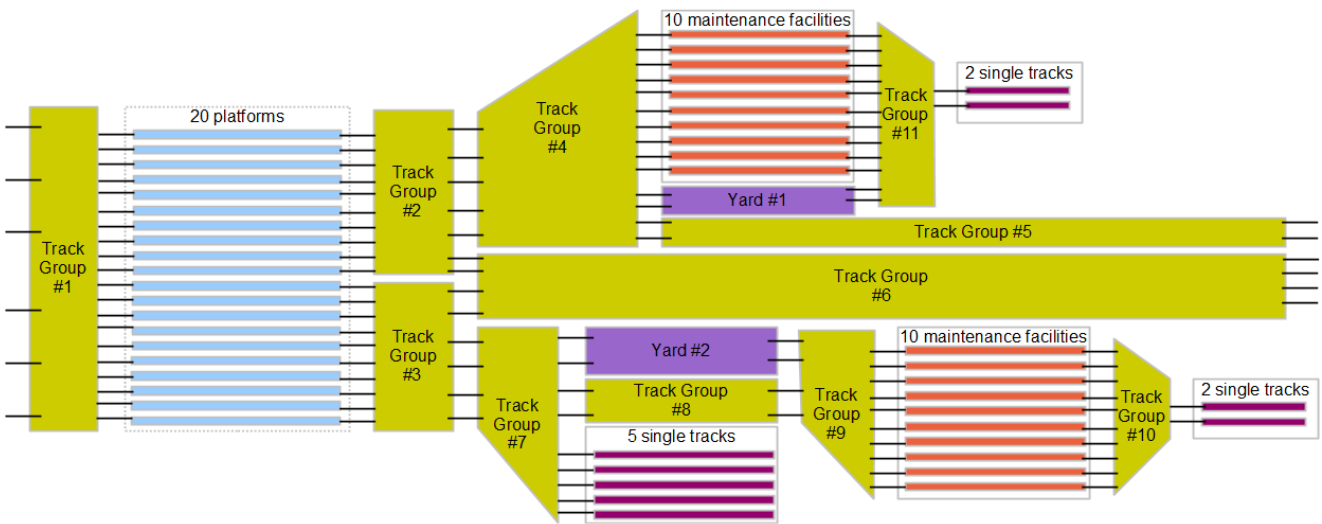
\includegraphics[width=12cm]{resources}
    \caption{Ejemplo de recursos de infraestructura (Fuente \cite{Problem})}
    \label{fig:resources}
    \end{figure}

    Es muy importante considerar la forma en que los trenes se mueven entre los recursos y sus restricciones. Los principales aspectos se listan como sigue:
    \begin{enumerate}
        \item Un mismo tren no puede estar ocupando dos recursos en el mismo instante de tiempo (algo que sí sucede en la realidad). Por lo tanto cada tren se considera como un objeto puntual que puede moverse de un recurso a otro de modo instantáneo.
        \item Cada recurso $r \in \mathcal{R}$ tiene un conjunto de recursos vecinos $\text{neighSet}_r$, que definen las posibles transiciones de un tren, esto es, un tren en un recurso $r$, sólo puede moverse a un recurso vecino en $\text{neighSet}_r$.
        \item Usualmente (hay excepciones) cada recurso puede ser accedido por dos lados, que se denotan A y B. Entonces el conjunto de recursos vecinos de $r$ puede ser descompuesto en $\text{neighSet}_r = \text{neighSet}_r^A \cup \text{neighSet}_r^B$. Adicionalmente se tiene como restricción $\text{neighSet}_r^A \cap \text{neighSet}_r^B = \emptyset$, esto es, que no se generen ciclos entre los recursos.
        \item Las excepciones al punto anterior las constituyen los recursos al extremo del sistema, por donde los trenes entran o salen.
        \item Los recursos tienen en ambos extremos \textit{puertas} por donde se realiza la transición hacia otro recurso.
        Cada puerta $g \in \mathcal{G}_r$ de un recurso $r$, está asociada a una única puerta de un recurso vecino (si la puerta está en el fin del sistema, puede no tener puerta vecina asociada).
        \item Las pistas simples, plataformas y instalaciones de mantención tienen como máximo una puerta en cada lado.
        \item Los grupos de pistas y estacionamientos pueden tener mas de una puerta en cada lado.
        \item Algunos recursos pueden ser utilizados sólo por un tipo específico de tren (por lo general en las estaciones de mantenimiento). Por ello cada recurso $r$ tiene su conjunto de categorías de trenes compatibles $\text{compCatRes}_r$.
        \item Pueden haber recursos ocupados con antelación en el sistema. Estos factores son externos al problema y fijos, siendo algunos ejemplos: trenes de mantenimiento, trenes que no terminan en la estación, trenes externos de otras compañías, entre otros.
    \end{enumerate}

    Teniendo una idea de la mecánica de uso de recursos del sistema, a continuación se entregan detalles específicos de cada tipo de recurso.
    \begin{enumerate}
        \item \textbf{Pistas Simples.} Corresponden a pistas unitarias, usada para el movimiento de los trenes dentro de la estación. Estos son (usualmente) los recursos que utilizan los trenes para entrar y salir del sistema. Cada pista simple $s \in \mathcal{S}$ tiene asociado un largo total $\text{lenght}_s$ y cantidad de trenes $\text{capa}_s$,
        que debe ser respetado en cada instante de tiempo.
        \item \textbf{Plataformas.} Estas representan las pistas en donde los pasajeros pueden salir o abordar un tren. Por lo tanto son estas, las que deben ser asignadas a cada llegada o salida respectivo. A diferencia de las pistas simples, una plataforma $p \in \mathcal{P}$ sólo está restringida en capacidad por su largo $\text{lenght}_p$.
        \item \textbf{Instalaciones de Mantenimiento.} Estas instalaciones son pistas donde los trenes se detienen a realizar su respectiva mantención (reajustar su TBM y DBM). Es muy importante notar que cada instalación de mantenimiento $f \in \mathcal{F}$ está equipada para hacer sólo un tipo de operación (``D'' o ``T''). Por lo tanto si un tren requiere hacer ambos mantenimientos, deberá pasar por dos instalaciones distintas. Por último, al igual que las plataformas, su capacidad está restringida por su largo $\text{lenght}_f$.
        \item \textbf{Grupos de Pistas.} Son un conjunto agregado de pistas, utilizados para mover a los trenes entre los distintos recursos del sistema. Todas las puertas de un lado son alcanzables desde el otro (y viceversa), por lo tanto si en un lado hay $m$ puertas y en el otro lado hay $n$, existen $m\ n$ posibles rutas para atravesar el grupo de pistas. Un grupo de pistas $k \in \mathcal{K}$ tiene dos parámetros importantes: el tiempo necesario para atravesar $k$ $\text{trTime}_k$ (constante), y el tiempo mínimo que debe haber entre dos trenes sucesivos para que no estén tan cerca $\text{hwTime}_k$. Técnicamente los grupos de pistas son una estructura compleja, que debe manejar normas de seguridad y conflictos que suelen ocurrir. Sin embargo el problema se abstrae de esta complejidad, viendo a tal estructura como una \textit{caja negra}.
        \item \textbf{Estacionamientos.} Al igual que el anterior, son también un conjunto de pistas pero utilizadas para estacionar trenes. Por lo tanto un tren puede permanecer en un estacionamiento sin limites de tiempo. Un estacionamiento $y \in \mathcal{Y}$ está limitado en capacidad por la cantidad de trenes permitidos $\text{capa}_y$.
    \end{enumerate}


    \item[\textsc{Objetivo.}] Tal como se plantea el problema, la objetivo general se descompone en múltiples objetivos,
    que corresponden a minimizar las penalizaciones descritas anteriormente. Luego la función a minimizar es:
    \begin{align}
        f = f^{\text{uncov}} + f^{\text{over}} + f^{\text{plat}} + f^{\text{pref}} + f^{\text{reuse}},
        \label{eq:gobj}
    \end{align}
    donde cada una representa:
    \begin{enumerate}
        \item $f^{\text{uncov}}$: Costo por no cubrir una salida.
        \item $f^{\text{over}}$: Costo asociado al sobre-mantenimiento.
        \item $f^{\text{plat}}$: Costo por uso de las plataformas.
        \item $f^{\text{pref}}$: Costo por no respetar la preferencia de uso de plataforma.
        \item $f^{\text{reuse}}$: Costo por no respetar un reuso dado inicialmente.
    \end{enumerate}
    un análisis más detallado de (\ref{eq:gobj}) será visto en la sección de Modelo Matemático.
    \item[\textsc{Solución Esperada.}] Como solución al problema, se espera una conjunto de programación de eventos
    para cada tren, esto es, una secuencia de eventos junto con los recursos usados, y los tiempos asociados. Los diferentes tipos de eventos pueden ser: \texttt{EnterSystem}, \texttt{ExitSystem}, \texttt{Arrival}, \texttt{Departure}, \texttt{EnterResource}, \texttt{ExitResource}, \texttt{BeginMaintenance} y \texttt{EndMaintenance}. Un ejemplo de posible solución para un tren dado se da en Figura \ref{fig:sched}.
     \begin{figure}[htpb!]
    \centering
    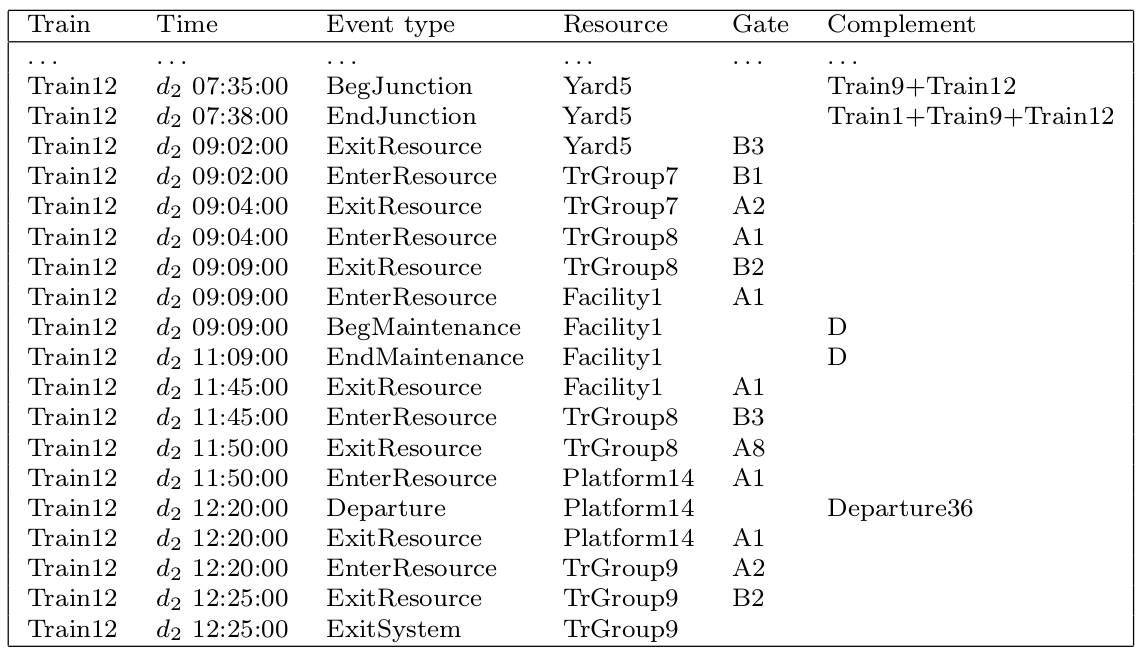
\includegraphics[width=12cm]{sched}
    \caption{Extracto de programación de eventos para un tren dado (Fuente \cite{Problem})}
    \label{fig:sched}
    \end{figure}
    Teniendo esta información para todos los trenes, será posible inferir el estado del sistema y sus recursos, en cada instante del horizonte de planificación.

\end{description}




\section{Estado del Arte} \label{SoA}
En la presente sección se hace un estudio acerca de cómo nace este problema y la forma en que ha sido abordado. Pese a que  hay gran cantidad de trabajo realizado (y en desarrollo) al respecto \cite{RoadefResults}, hay pocos que han sido publicados. Por lo tanto también se expondrán las variantes o sub-problemas más conocidos, así como los distintos enfoques con los que han sido abordados.

\begin{description}
    \item[\textsc{Inicios del Problema.}] En el problema de estudio en el presente artículo, corresponde a una versión \textit{simplificada} del problema propuesto en el ROADEF/EURO Challenge 2014 \cite{Problem}, competencia organizada
    por la \textit{SFrench Operational Research (OR) and Decision Support Society} (ROADEF) y la \textit{European Operational Research Society} (EURO) en conjunto con la \textit{Société Nationale des Chemins de Fer Français} (SNFC).
    El objetivo de esta, fue encontrar la mejor forma realizar el manejo, ruteo y asignación de trenes en una estación ferroviaria, tal como se explicó en la sección \ref{probdef}. La simplificación nombrada, consiste en que se da por alto una de las dimensiones del problema, que es la unión y separación de trenes. Como se explicó en la sección \ref{probdef},
    los trenes son las unidades de asignación más pequeñas a utilizar, esto es, no pueden ser separados ni recombinados sus vagones. Sin embargo, en la medida de poder satisfacer salidas con gran cantidad de pasajeros, es posible \textit{unir}
    dos trenes en el sistema para cumplir con la capacidad. El proceso de \textit{unir} y \textit{separar} trenes en las estaciones es llevado en los \textit{grupos de pistas}, y agrega una complejidad considerable a la formulación y a su solución.
    Una buena cantidad de equipos lograron dar con soluciones satisfactorias \cite{RoadefResults}. Algunas de estas se detallan en lo que sigue.

    \item[\textsc{Propuestas de Solución.}]
    El primer trabajo publicado corresponde a \textit{A Math-Heuristic Framework for the ROADEF/EURO Challenge 2014} \cite{MathHeuristic}, cuyos autores participaron en la categoría junior del concurso obteniendo el segundo lugar. El nombre \textit{math-heuristic} se debe a que se combinan métodos exactos con heurísticas para hallar una solución. El problema original se aborda como cuatros sub-problemas, tal como se describe en la figura \ref{fig:diagram}. Cada etapa se resume a continuación:
    \begin{enumerate}
        \item \textsc{Arrival\&Departure Matching}. En esta primera etapa, se intenta hacer un \textit{match} para cada salida, con un tren compatible (tren inicial o de llegadas). El problema es planteado como MIP (\textit{Mixed Integer Programming}), con básicamente dos objetivos: Minimizar el número de cancelaciones de salidas (salidas sin cubrir) y maximizar la cantidad de reusos entre las llegadas y salidas. Debido a la gran cantidad de variables involucradas, este es resuelto usando el método de generación de columnas. Para generar los \textit{matches} se generan los conjuntos $\text{Comp}(d)$ y $\text{Comp}(t)$ que contienen los trenes compatibles para cada salida $d$ y las salidas compatibles a cada tren $t$, respectivamente. Estos se computan filtrando las combinaciones inviables, y utilizando heurísticas (eg. eliminando \textit{matches} en espacios de tiempo muy grandes).
        \item \textsc{Platform Assignment}. En segundo lugar es necesario asignar las plataformas a utilizar por cada llegada y salida a cubrir. Se intenta aquí asignar de manera que se minimicen las cancelaciones de llegada y salidas, y que cada una sea asignada a su plataforma preferida, en la medida de lo posible. Este también se plantea como MIP, pero se resuelve buscando una solución exacta.
        \item \textsc{Arrival\&Departure Sequence Assigner}. Luego para cada una de las llegadas y salidas a cubrir, se generan patrones de uso de los grupos de pistas, de modo que no existan conflictos entre en las secuencias respectivas, ni el uso de recursos impuestos inicialmente.
        \item \textsc{Simulated Annealing / Train Routing}. En última instancia, \textit{Simulated Annealing} (SA) es utilizado para generar rutas (secuencia de recursos) que los trenes realizan en la estación. Para ello en cada iteración se \textit{rutea} a un tren, seleccionando una ruta aleatoria basada en los \textit{matches} y asignación de recursos anteriores. Cada nueva solución es aceptada dependiendo del costo y temperatura.
    \end{enumerate}
    Cabe mencionar el este artículo no trabaja las condiciones de uniones de trenes en llegadas y salidas. En definitiva este enfoque se basa en ocupa SA para generar rutas aleatorias, apoyándose en resultados precomputados para la utilización de recursos y evitar conflictos.
    \begin{figure}[htpb!]
    \centering
    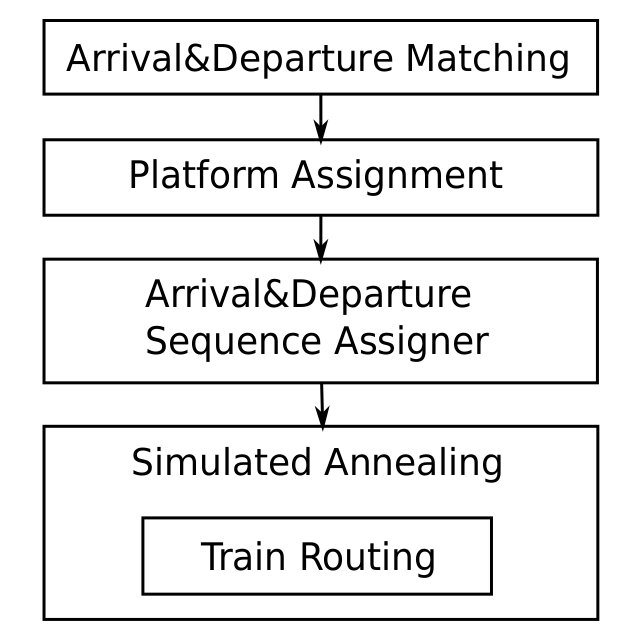
\includegraphics[width=4cm]{diagram}
    \caption{Esquema de solución en Math-Heuristic Framework (Fuente \cite{MathHeuristic})}
    \label{fig:diagram}
    \end{figure}

    El segundo trabajo \textit{Roadef Challenge 2014: A Modeling Approach, Rolling stock unit management on railway sites}\cite{ModelingApproach}, presenta un acabado estudio con un modelo similar al anterior; Descompone el problema original en dos etapas de decisión: asignación y enrutamiento. La idea de generar estos dos subproblemas, es reducir la complejidad inicial, y ocupar la técnica de resolución indicada para cada uno. Por un lado, la primera etapa se compone básicamente de asignar trenes (de las llegadas o inicialmente en el sistema) a las salidas, asignar plataformas, y el resto de recursos del sistema. Este tipo de problemas son fácilmente formulables en MIP, y pueden ser resueltos de manera eficiente con dicha representación (por generación de columnas). Por otro lado, la fase de enrutamiento de trenes en la estación se desacopla totalmente de la fase de asignación, y se propone utilizar CP (\textit{Constraint Programming}) para su solución, pues es la opción más viable y eficiente. Algunos detalles se listan a continuación para cada fase (Ver Figura \ref{fig:diagram2}).
     \begin{figure}[htpb!]
    \centering
    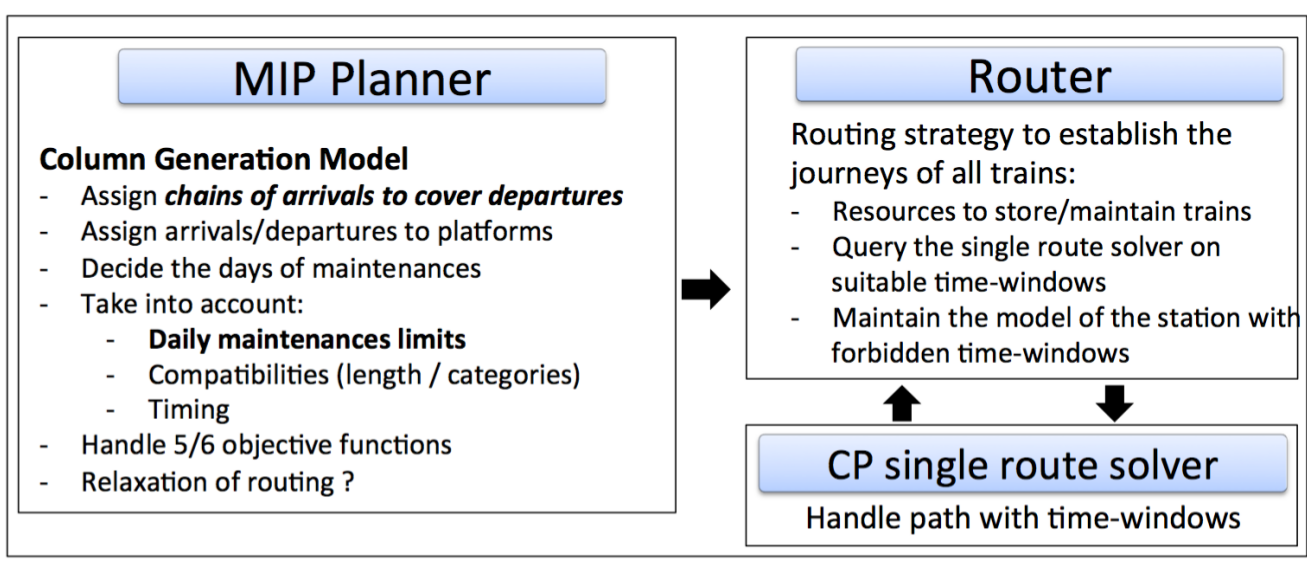
\includegraphics[width=8cm]{diagram2}
    \caption{Esquema de solución de Modeling Approach (Fuente \cite{ModelingApproach})}
    \label{fig:diagram2}
    \end{figure}

    \begin{enumerate}
        \item \textsc{Asignación.} El problema de asignación abarca asignar trenes a las salidas, asignar plataformas a las llegadas y salidas y asignar las mantenciones. La función objetivo que se plantea planteada considera: \textit{llegadas/salidas no cubiertas}, \textit{trenes iniciales no usados}, \textit{plataformas preferidas no satisfechas}, \textit{reusos no satisfechos} y \textit{sobre mantenciones}. Todo lo anterior se modela por medio de MIP. Se hace luego una extensión a esta formulación para considerar el caso de llegadas \textit{enlazadas} con salidas previas, verificando que tal problema se reduce a \textit{Dependent Matching Problem} (DPM) que es NP-completo.  
        \item \textsc{Enrutamiento.} Para esta se parte de la premisa de que es posible computar las rutas de los trenes en la estación, sin cuestionar los resultados previos de la fase de asignación. Aquí modela la estación y sus recursos como un grafo, y muestra que el problema de enrutar un sólo tren se reduce a \textit{Resource Constrained Shortest Path Problem} (RCSPP) que es NP-hard. En base a esto, un modelo de CP es inferido para definir las rutas, y luego se computan una por una las rutas de todas las llegadas/salidas, de modo que si el \textit{solver} de CP es incapaz de encontrar una solución, se cancela la llegada/salida asociada.
    \end{enumerate}
    Los autores reconocen que uno de los puntos débiles del modelo propuesto está en la estrategia de enrutamiento, sobre la cual es posible usar distintas heurísticas para tratar el problema de formas más integrada, y así minimizar las cancelaciones.

    Un estudio interesante es el que realiza (nuevamente) Haahr et al. \cite{Haahr}, en donde se enfocan en la tarea de analizar, modelar y solucionar uno de los subproblemas de \textit{Rolling Stock Unit Management on Railway Sites Problem} (RSUM) más importantes; El \textit{train Departure Matching Problem} (DMP), que consiste en realizar las asignaciones de trenes (entre los que están inicialmente, y los de las llegadas) a las correspondientes salidas, satisfaciendo las restricciones de compatibilidad y mantenciones. La importancia del DPM subyace en que cualquier enfoque utilizado para solucionar el RSUM, se ve afectado en gran parte por cómo los trenes son asociados a las salidas. En primer lugar se muestra que el DMP es NP-hard por reducción al \textit{0-1 Multiple Knapsack Problem}. Luego se propone resolver el problema con métodos exactos, formulando el problema como MIP (\textit{Mixed Integer Programming}) de dos formas equivalentes; La primera de ellas es resulta con el MIP \textit{solver} IBM ILOG CPLEX, y la segunda con métodos de generación de columnas. En las pruebas ambos métodos demoran una gran tiempo en computar sus soluciones. Para ello propone se proponen heurísticas para generar columnas, eliminando las columnas innecesarias en el modelo anteriores.

    La tesis de Mulders y Scholliers \cite{Mulders} constituye un análisis en detalle respecto al problema. A modo de estudio preliminar, se modela inicialmente el problema con tres enfoques distintos. El primero de ellos es plantear las asignaciones de salidas a trenes como un \textit{Matching} en un grafo bipartito, la segunda ocupa \textit{constraint programming} restringiendo las posibles configuraciones, y la tercera se plantea resolver mediante greedy. El cómputo de las rutas que siguen los trenes en el sistema, se hace a traves de MIP con LPsolve. Pese a que los tres enfoques sufren de serios problemas en cuanto a tiempo de computación (no son factibles de utilizar), su análisis ayudó a desarrollar la solución final. Esta última posee cuatro componentes principales:
    \begin{enumerate}
        \item \textbf{Objects}, que corresponden a una representación conveniente (para esta formulación) de los datos y variables del sistema.
        \item \textbf{Oracle}, es un componente encargado de verificar que distintas acciones puedan ser llevada a cabo sin violar restricciones, así como determinar donde y cuando pueden ser llevadas a cabo (mantenciones por ejemplo).
        \item \textbf{WaysPC}, que es capaz de computar rutas compatibles para todos los trenes presentes en el sistema en un instante dado.
        \item \textbf{Solver}, componente principal que hace uso de los anteriores, para encontrar soluciones usando una metodología greedy.
    \end{enumerate}
    El objetivo principal del solver propuesto es dejar la menor cantidad de partida sin asignar, esto pues por ejemplo, es mucho más importante cubrir una partida que asignarla a una plataforma no preferida. En la Figura \ref{fig:graphres} se
    muestra el porcentaje de partidas cubiertas en un horizonte de $7$ días, para $6$ distintas instancias del desafío. Se puede notar que el desempeño de las asignaciones va empeorando en el tiempo.
    \begin{figure}[htpb!]
    \centering
    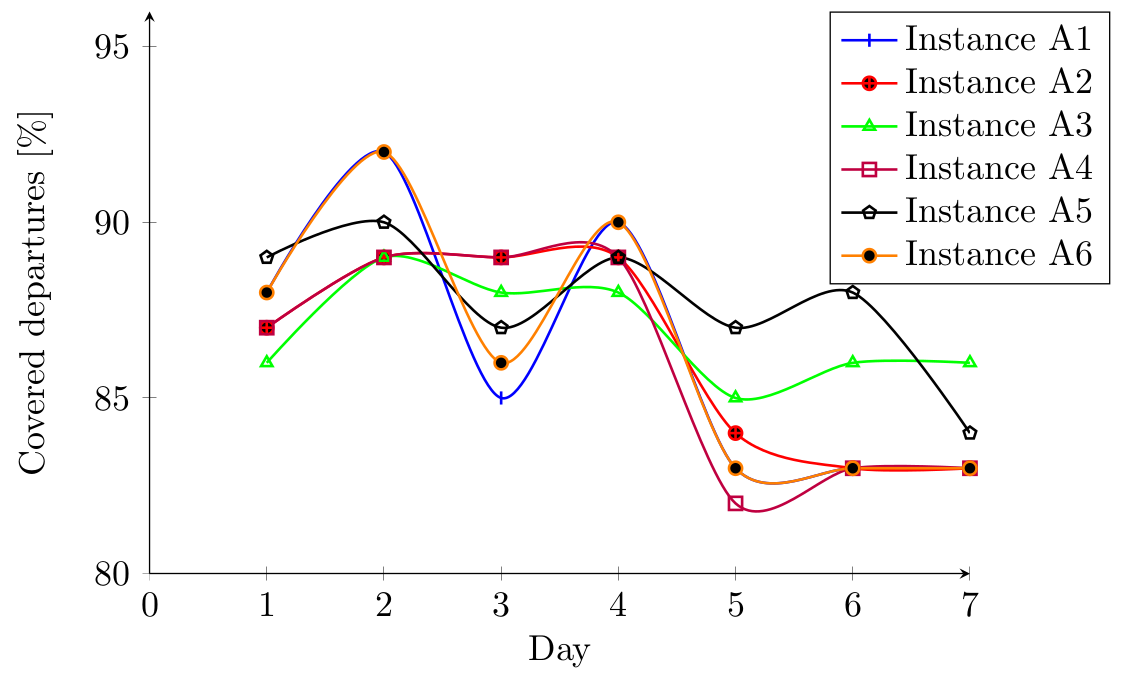
\includegraphics[width=9cm]{graphres}
    \caption{Porcentaje de salidas asignadas por Solver (Fuente \cite{Mulders})}
    \label{fig:graphres}
    \end{figure}
    Los autores concluyen que el algoritmo desarrollado, es de hecho competitivo, pues es capaz de entregar soluciones a instancias del ROADEF/EURO Challenge 2014 en menos de un minuto (el tiempo límite para estas instancias era de $10$ minutos). Por otro lado obtiene desempeños similares a las mejores soluciones del desafío \cite{RoadefResults}. Por último se propone como trabajo futuro, determinar heurísticas que permitan mejorar aún más la calidad de las soluciones, así como mejorar la definición de los objetivos en el modelo.




    \item[\textsc{Problemas Relacionados.}] El problema en estudio ha sido estudiado y abordado múltiples maneras; Distintos objetivos, restricciones y metodologías de solución. En el presente estudio, se presentan las más notables entre estas.

    Uno de los principales sub-problemas es conocido como \textit{Train Timetabling Problem}, el cual consiste en generar una planificación horaria para los trenes en una estación, para cubrir las salidas satisfaciendo restricciones particulares del sistema. Este problema ha sido modelado y resuelto mediante múltiples técnicas. Uno de los primeros estudio formales lo entrega Caprara \cite{Caprara}, quien modela el problema y demuestra que es NP-hard, siendo una generalización del MSSP (\textit{Maximum Stable Set Problem}).

    Una solución al TTP en con una sola pista es propuesta por Cacchiani et al. \cite{Cacchiani}, basado en método de generación de columnas. Aquí se propone un modelo de ILP (\textit{Integer Linear Programming}) en donde cada variable, corresponde a la secuencia de programaciones horarias de un tren, denominadas \textit{path variables} (variables de ruta). Esto genera una gran cantidad de combinaciones y posibles soluciones, por lo tanto es adecuado de resolver con técnicas generación de columnas. Adicionalmente un método basado en heurísticas y \textit{local search} es propuesto e implementado. Ambas propuestas fueron probadas con instancias reales de \textit{Rete Ferroviaria Italian} (RFI). Los resultados mostraron que pese a que el número de variables de la primera formulación crece exponencialmente, estos son resueltos en tiempos razonables. Por otro el modelo basado en heurísticas entrega mejores resultados, sin embargo los tiempos de computación son considerablemente mayores.

    Una variante interesante propone Mohammad et al. \cite{Mohammad} en la resolución del TTP con una sola vía. Se formula el modelo como MIP, con la capacidad de manejar pequeñas perturbaciones en las llegadas y salidas de trenes, lo cual ocurre regularmente en la realidad. Para eso introduce variables que manejar el tiempo de \textit{buffer}, los cuales se modelan de dos formas: Con una distribución conocida de las perturbaciones y con distribución desconocida. Para la resolución se utiliza en \textit{Branch and Bound} (BB), y se propone una heurística \textit{Beam Search} (BS) para encontrar soluciones factibles en tiempos en tiempos razonables. Para verificar la validez del método basado en BB, se comparan con los resultados que entrega el software \texttt{Lingo}. Los resultados muestran que para todas las instancias pequeñas los resultados coinciden, sin embargo ninguno es capaz de resolve instancias muy grandes. Por otro lado el método basado en BS entrega buenos resultados para las instancias pequeñas (y en menor tiempo), y es capaz de determinar soluciones factibles para las instancias en que los otros dos no pueden.  


    Por otro lado Tormos et al. \cite{Genetic} también propone resolver el TTP en una sóla pista simple, pero mediante algoritmos genéticos (GA por \textit{Genetic Algorithm}). La elección de este método es que el problema posee un espacio de búsqueda complejo, y precisamente los GA son capaces de llegar a buenas soluciones y en poco tiempo en tales casos. El problema se limita al estudio de pistas simples, con secciones dobles. Para cada nuevo tren se define su \textit{traversal time}, que consiste en el menor tiempo en que puede atravesar la estación sin violar restricciones del sistema. Luego la función objetivo se define como la suma de tales tiempos. El algoritmo genético que se propone se basa en modelo utilizado en \textit{Job-Shop Scheduling Problem}, en donde se genera una programación de trabajos, los cuales satisfacen restricciones de tiempo y recursos, con el menor esfuerzo posible y en el menor espacio de tiempo. Para el proceso se utilizan y definen operaciones de \textit{crossover} (cruzamiento), \textit{mutation} (mutación) y \textit{selection}, usando heurísticas para definir la población inicial. La propuesta se prueba en instancias reales obtenidas del ADIF (Administrador de Infraestructura Ferroviaria) de España. Los resultados muestran que el método propuesto permite obtener resultados factibles en tiempos relativamente bajos (minutos), lo cual es bueno considerando el gran tamaño de las instancias.

    Un buen sumario acerca del TTP en sola vía lo provee Higgins et al. \cite{Higgins}. En este se explica la importancia de utilizar heurísticas para este tipo de problemas, en donde encontrar óptimos globales no es una posibilidad. Para ellos se prueba con \textit{Local Search Heuristics} (heurísticas de búsqueda local, LSH), Algoritmos Genéticos (GA), Tabu Search (TS) y dos algoritmo híbridos (HA1 y HA2). Una consideración importante del modelo a utilizar, es que supone que las llegadas y salidas no son conocidas de un inicio (no son datos iniciales), y por lo tanto tienen la libertad de ser planificadas. Las algoritmos híbridos recién nombrados, tienen como propósito combinar las ventajas de dos o más heurísticas. En la primera variante (HA1) combina GA con LSH, de modo que en cada iteración de GA (antes de la operación de \textit{crossover}) se realiza LSH sobre el $5\%$ mejor de la población, ayudando de este modo a que GA alcance convergencia más rápido. La segunda variante (HA2) combina GA con TS para mejorar el proceso de \textit{crossover}, permitiendo elegir padres y posiciones de cruzamiento que no produzcan descendencia en la próxima generación. En la Figura \ref{fig:rescomp} puede apreciarse una comparación de los resultados obtenidos para cada algoritmo, donde los valores que se muestran corresponden al tiempo de viaje (en estación) con pesos    promediados sobre $20$ ejecuciones en cada instancia (valores más bajos son mejores). En la tabla se aprecia que los algoritmos híbridos obtienen por lejos mejores resultados, siendo H2 el mejor entre ambos. La heurística con peor desempeño fue LSH, debido a su poca capacidad de escapar de óptimos locales.
     \begin{figure}[htpb!]
    \centering
    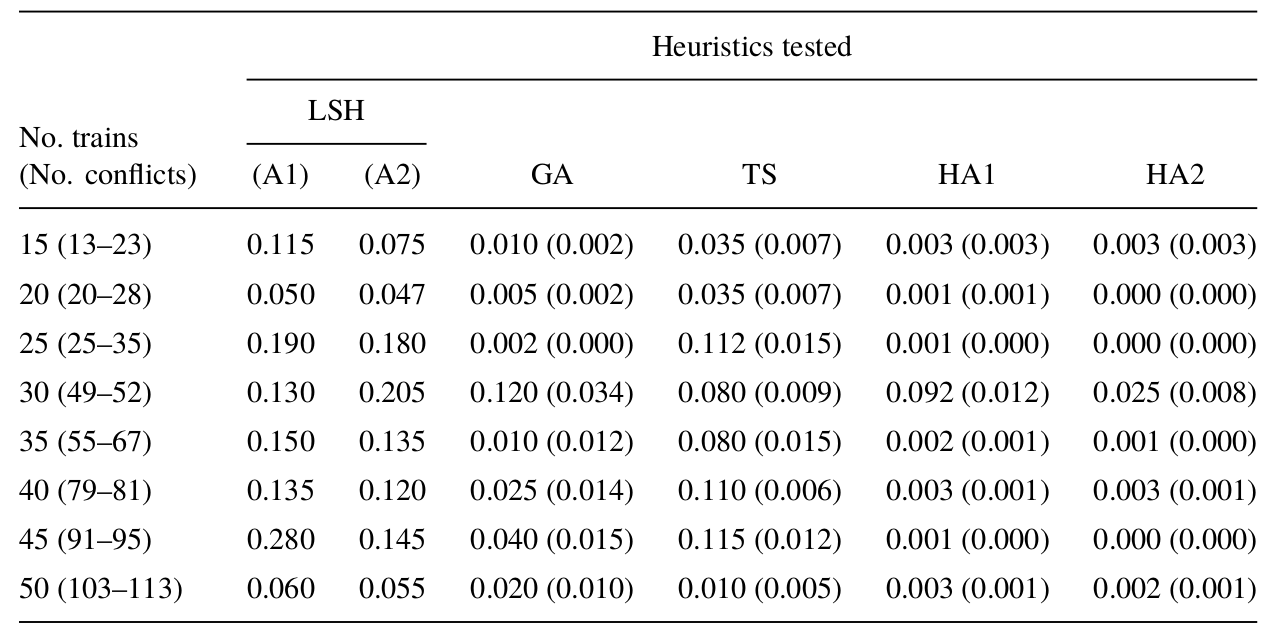
\includegraphics[width=9cm]{rescomp}
    \caption{Comparación de resultados de Heurísticas (Fuente \cite{Higgins})}
    \label{fig:rescomp}
    \end{figure}
    Por otro lado en la Figura \ref{fig:timecomp} se hace una comparación de la capacidad de mejora de la solución, versus los tiempos de procesamiento para cada heurística (se agrega \textit{Branch and Bound} que fué el método para computar la solución óptima). Se puede apreciar que GA, HA1 y HA2 no son capaces de determinar soluciones antes de los $35$ segundos, esto pues primero deben computar la población inicial. Sin embargo luego de computada esta, la razón de convergencia de HA1 y HA2 es superior a la del resto. Por otro lado, se nota que TS y LSH convergen rápido en un inicio, pero luego se estancan. Se termina concluyendo que los algoritmos híbridos son los más viables, y con el mejor desempeño general.

    Otra variante del problema, la constituyen el \textit{Train Rescheduling Problem} en el cual se deben resolver conflictos en tiempo real. Esta es una situación común, en la cual debido a imprevistos (accidentes, retrasos, etc) la planificación prevista debe ser modificada, para poder satisfacer las llegadas/salidas con la menor variación posible. La dificultad se encuentra en realizar una re-planificación aceptable, en el menor tiempo posible. En el trabajo realizado por Norio et al. \cite{Norio}, se propone un modelo de \textit{rescheduling} que intenta minimizar la insatisfacción de la gente. El algoritmo propuesto combina \textit{Program Evaluation and Preview Technique} con el método de \textit{Simulated Annealing}. De modo similar D'Ariano et al. \cite{DAriano} afrontan el mismo problema, pero utilizando el método de \textit{Branch and Bound} (BB). Debido a las restricciones de tiempo, el proceso de BB es acelerado ocupando \textit{reglas de implicación estáticas}, que explotan las propiedades de las soluciones factibles. Las pruebas muestran que el método propuesto es capaz de computar soluciones óptimas (o cercanas) en tiempos pequeños.

    Un problema con mayor parecido al que se trata aquí, es el \textit{Multi Objective Train Scheduling Problem}. El problema tratado por Ghoseiri et al \cite{Ghoseiri} se asemeja bastante al de este estudio, en cuanto a las estructura que considera: Una red de pistas compuestas por pistas simples, múltiples pistas, múltiples plataformas (con capacidad de movilidad entre ellas), y múltiples plataformas con distinta capacidad. Sin embargo los objetivos que se plantea son: 1) Minimizar la utilización de combustible (medida de eficiencia que aumenta satisfacción de compañía) y 2) minimizar el tiempo de los pasajeros (medida de eficacia que aumenta la satisfacción de pasajeros). Una formulación diferente la plantea Li et al. \cite{Li}, considerando en sus objetivos: 1) Minimizar la cantidad de energía utilizada, 2) Minimizar los costos de emisiones de carbón, y 3) Minimizar el tiempo de los pasajeros. Debido a sus objetivos, sus autores llaman al modelo \textit{green train scheduling problem}.   

    \begin{figure}[htpb!]
    \centering
    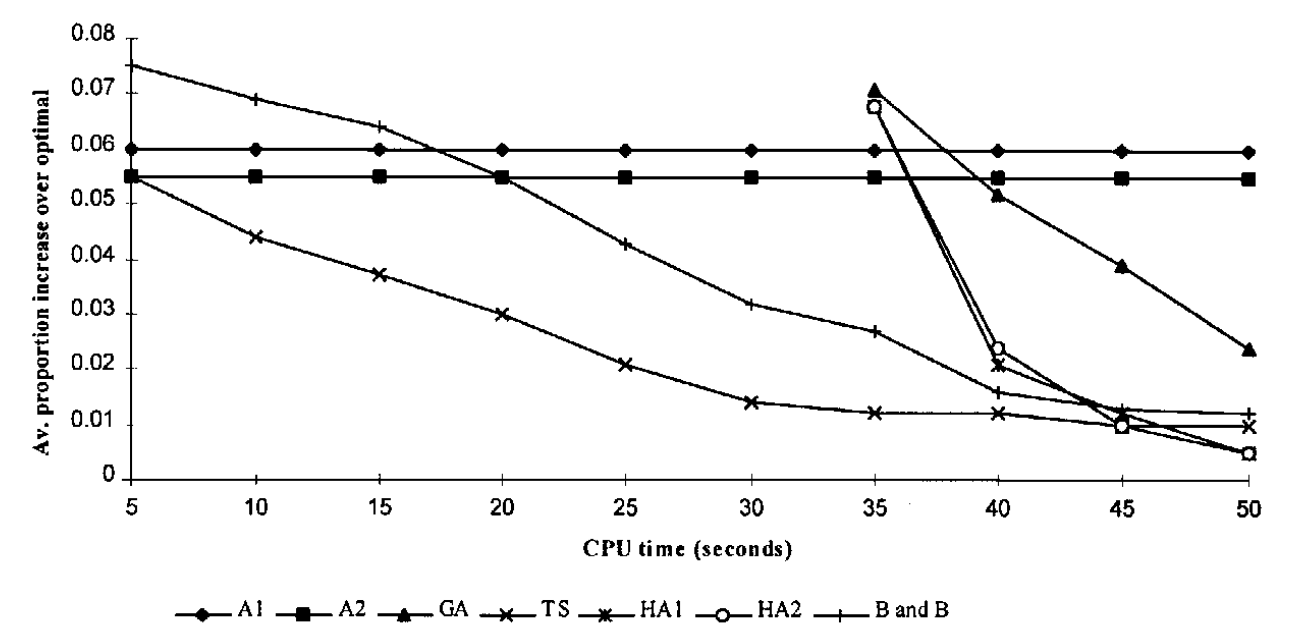
\includegraphics[width=9cm]{timecomp}
    \caption{Comparación de convergencia versus tiempo de ejecución de Heurísticas (Fuente \cite{Higgins})}
    \label{fig:timecomp}
    \end{figure}
\end{description}

\section{Modelo Matemático} \label{model}
A fin de mantener la definición del problema simple en la Sección \ref{probdef}, muchas notación y aspectos técnicos fueron omitidos. En lo que sigue se pretende dar una descripción formal más acabada al respecto. La formulación propuesta sigue la descripción del problema en \cite{Problem}, con pequeñas modificaciones equivalente para facilitar la comprensión. Por lo tanto se ocupa la misma notación para mantener la coherencia. Para no abrumar al lector, la notación se explica de modo progresivo (en la medida que se requiera).

\subsection{Restricciones}

\begin{description}
    \item \textsc{Propiedades de las Programaciones.}
    \begin{enumerate}
        \item \textbf{Entradas en el sistema.}
        \begin{align*}
            \mathcal{A} &:= \ \text{Conjunto de llegadas.} \\
            \mathcal{T}_I &:= \ \text{Conjunto de trenes inicialmente en el sistema.} \\
            \mathcal{T}_A &:= \ \text{Conjunto de trenes que ingresan por una llegada } a \in \mathcal{A} \\
            \mathcal{T} &:= \ \text{Conjunto de todos los tres: } \mathcal{T}_I \cup \mathcal{T}_A \\
            \mathcal{T}^{+} &:= \ \text{Conjunto de trenes usados en al solución.} \\
            \text{arrSeq}_a &:= \ \text{Secuencia de llegada para } a \in \mathcal{A}. \\
            \text{arrTime}_a &:= \ \text{Tiempo de llegada a una plataforma para } a \in \mathcal{A}. \\
            \text{res}_t &:=\ \text{Recurso ocupado por un tren } t \text{ inicialmente en el sistema}
        \end{align*}
        Para todos los trenes $t \in \mathcal{T}_I$, los eventos \texttt{EnterSystem} y \texttt{EnterResource},
        deben ocurrir en el instante inicial del horizonte $\text{d}_1 \ 00:00:00$, en el recurso inicial $\text{res}_t$. Para los trenes asociados a llegadas $t \in \mathcal{T}_A$, el evento \texttt{EnterSystem} de ser procedido inmediatamente (mismo instante) por un \texttt{EnterResource} en un conjunto de pistas, seguido por un \texttt{ExitResource} de acuerdo a su secuencia de llegada $\text{arrSeq}_a$. El evento \texttt{EnterResource} en la plataforma debe ocurrir al instante $\text{arrTime}_a$.

        \item \textbf{Salidas del sistema.}
        \begin{align*}
            \mathcal{D} &:= \ \text{Conjunto de salidas.} \\
            \text{depSeq}_d &:= \ \text{Secuencia de salida de } d \in \mathcal{D}. \\
            \text{depTime}_d &:= \ \text{Hora de salida de la plataforma de } d \in \mathcal{D}. \\
            \text{d}_{\text{nbDays}} &:= \ \text{Número de días considerados en el horizonte.}
        \end{align*}
        La programación para todo $t \in \mathcal{T}^+$ debe terminar en un evento \texttt{ExitSystem}. Si el tren $t$ no se asigna a una salida, tal evento debe ocurrir al instante final del horizonte $\text{d}_{\text{nbDays}} \ 23:59:59$ (precedido por el \texttt{ExitResource} respectivo). Un tren asociado a una salida $d \in \mathcal{D}$ debe realizar un \texttt{ExitResource} al instante $\text{depTime}_d$, seguido por una serie de \texttt{EnterResource} y \texttt{ExitResource} en los conjuntos de pistas impuestos por la secuencia de salida $\text{depSeq}_d$.

        \item \textbf{Uso de un recurso.}
        \begin{align*}
            \mathcal{E} &:= \ \text{Conjunto de posibles eventos.} \\
            r_e &:= \ \text{Recurso utilizado por el evento } e \in \mathcal{E}. \\
            \text{sched}_t &:= \ \text{Secuencia de eventos asociadas al tren } t \in \mathcal{T}^+.
        \end{align*}
        Cada evento \texttt{EnterResource} $e$ en $\text{sched}_t$, debe ser seguido por un evento $e'$ del tipo \texttt{ExitResource}, tal que $r_e = r_{e'}$ (asociados al mismo recurso). Entre $e$ y $e'$ sólo puede ocurrir eventos de tipo \texttt{Arrival}, \texttt{Departure} y \texttt{Beg/EndMaintenance}, con recurso asociado $r_e$.


        \item \textbf{Transición a un recurso vecino.}
        \begin{align*}
            g_e &:= \text{Puerta de entrada/salida al recurso } r_e \text{ para el evento } e \in \mathcal{E}. \\
            \text{neigh}_g &:= \text{Puerta vecina de g (da paso a otro recurso)}. \\
            h_e &:= \text{Instante en el horizonte } \mathcal{H} \text{ donde ocurre el evento.}
        \end{align*}
        Cada evento \texttt{ExitResource} $e$, debe ser \textit{seguido inmediatamente} por un evento $e'$ \texttt{ExitSystem} (si se encontraba en el recurso al borde del sistema), o un \texttt{Enter Resource} con $r_e \neq r_{e'}$ (recurso diferente). También debe cumplirse que $\text{neigh}_{g_e} = g_{e'}$. Seguido inmediatamente significa $h_e = h_{e'}$.

        \item \textbf{Operaciones de mantención.}
        \begin{align*}
            \mathcal{F} &:= \text{Conjunto de instalaciones de mantenimiento.} \\
            \text{maintTimeD}_t &:= \text{tiempo que demora el tren } t \text{ en realizar mantención tipo D.} \\
            \text{maintTimeT}_t &:= \text{tiempo que demora el tren } t \text{ en realizar mantención tipo T.} \\
            c_e &:= \text{Cuando } e \text{ involucra un recurso en } \mathcal{F}, \text{ esta indica el tipo de mantención.}
        \end{align*}
        Si el $\text{sched}_t$ de un tren $t \in \mathcal{T}^+$ contiene un evento \texttt{BegMaintenance}, entonces debe ser seguidos por eventos \texttt{EnterResource} y \texttt{ExitRosource} en alguna $f \in \mathcal{F}$,  tal que $\text{type}_f = c_e$, y debe finalizar con el evento \texttt{EndMaintenance} $e'$ cumpliendo:
        \begin{align*}
            c_e = D \Rightarrow h_{e'} = h_e + \text{maintTimeD}_t \\
            c_e = T \Rightarrow h_{e'} = h_e + \text{maintTimeT}_t.
        \end{align*}
        Notar que cada tren puede realizar a lo más una mantención de cada tipo (puede no realizar ninguna).
        \item \textbf{Uso de un grupo de pistas.}
        \begin{align*}
            \mathcal{K} &:= \ \text{Conjunto de grupos de pistas del sistema.} \\
            \text{trTime}_k &:= \ \text{Tiempo que toma recorrer } k \in \mathcal{K}. \\
            \text{side}_g &:= \text{Lado (A o B) asociado a la puerta g.}
        \end{align*}
        Un tren $t \in \mathcal{T}^+$ que realiza un evento $e$ \texttt{EnterResource} en un grupo de pistas $k$, debe ser seguido por un evento $e'$ \texttt{ExitResource}, cumpliendo:
        \begin{align*}
            h_{e'} &= h_e + \text{trTime}_k \\
            \text{side}_{g_{e'}} &\neq \text{side}{g_{e}}.
        \end{align*}
        \item \textbf{Mínimo tiempo de reversa.} Un tren $t \in \mathcal{T}^+$ que realiza un evento \texttt{EnterResource} sobre un recurso $r \in \mathcal{S}, \mathcal{P}, \mathcal{F} \text{ o } \mathcal{Y}$, debe ser seguido por un evento $e'$ \texttt{ExitResource} satisfaciendo:
        \begin{align*}
             \text{side}_{g_{e'}} = \text{side}_{g_e} \Rightarrow h_{e'} \geq h_e + \text{revTime},
          \end{align*}
          dónde $\text{revTime}$ es el tiempo que le toma a la tripulación, cambiar el sentido del viaje (caminar hacia el otro extremo del tren).
    \end{enumerate}

    \item \textsc{Asignaciones.}
    \begin{enumerate}
        \item \textbf{Restricciones de trenes.} Para cada salida $d \in \mathcal{D}$, esta debe ser asociada con a lo más un tren $t \in \mathcal{T}$.
        \item \textbf{Restricciones de DBM.}
        \begin{align*}
            \text{depTrain}_d &:= \ \text{Tren asociado a las salida } d. \\
            \text{reqDBM}_d &:= \ \text{DBM requerido para poder efectuar la salida} d. \\
            \text{remDBM}_t &:= \ \text{DBM restante para el tren t.} \\
            \text{maxDBM}_t &:= \ \text{DBM que alcanza un tren } t \text{ luego de operación de tipo D}. \\
            \text{linkedDep}_a &:= \ \text{La llegada } a \text{ esta asociada a la salida previa } d.   
        \end{align*}
        La restricción para que una salida sea factible es:
        \begin{align*}
            \text{Si } \ \text{depTrain}_d = t \Rightarrow \text{remDBM}_t \geq \text{reqDBM}_d
        \end{align*}
        En caso de que una llegada $a \in \mathcal{A}$, este enlazada $\text{linkedDep}_a = d$ con $\text{depTrain}_d = t$ y $\text{arrTrain}_a = t'$, entonces para actualizar el DBM y TBM se computa:
        \begin{align*}
            \text{remDBM}_{t'} = \text{remDBM}_t - \text{reqDBM}_d \\
            \text{remTBM}_{t'} = \text{remTBM}_t - \text{reqTBM}_d \\
        \end{align*}

        \item \textbf{Restricciones de TBM.}
        \begin{align*}
            \text{reqTBM}_d &:= \ \text{TBM requerido para poder efectuar la salida} d. \\
            \text{remTBM}_t &:= \ \text{TBM restante para el tren t.} \\
            \text{maxTBM}_t &:= \ \text{DBM que alcanza un tren } t \text{ luego de operación de tipo D}.   
        \end{align*}
        Análogamente, para que una salida $d$ sea factible debe cumplir:
        \begin{align*}
            \text{Si } \ \text{depTrain}_d = t \Rightarrow \text{remTBM}_t \geq \text{reqTBM}_d.
        \end{align*}

        \item \textbf{Compatibilidad de categoría.}
        \begin{align*}
            \text{cat}_t &:= \ \text{Categoría a la que pertenece el tren t.} \\
            \text{CompCatDep}_d &:= \ \text{Categoría de trenes compatibles para realizar la salida } d.
        \end{align*}
        La restricción es $\displaystyle \forall d \in \mathcal{D}, \forall t \in \mathcal{T}^+, \text{ si } \text{depTrain}_d = t \Rightarrow \text{cat}_t \in \text{compCatDep}_d$.
    \end{enumerate}

    \item \textsc{Utilización de Recursos.}
    \begin{align*}
        \text{use}_{t,h} &:= \text{Indica el recurso } r \text{ del que hace uso el tren } t \text{ en el instante } h. \\
        \text{nbTrain}_{r,h} &:= \text{Para } r \in \mathcal{S}\cup \mathcal{Y}, \text{ indica la cantidad de trenes haciendo uso de él.} \\
        \mathcal{I} &:= \text{Conjunto de utilizaciones impuestas con anticipación.} \\
        \text{res}_i &:= \text{Recurso (estacionamiento) utilizado por } i \in \mathcal{I}. \\
        \text{nb}_i &:= \text{Número de slots/trenes utilizados por } i \in \mathcal{I}. \\
        (\text{beg}_i,\text{end}_i) &:= \text{Instantes de inicio y término de } i \in \mathcal{I}.
    \end{align*}
    Notar que para las pistas simples se cumple:
    \begin{align*}
        \forall h \in \mathcal{H}, \forall r \in \mathcal{S}, \ \text{nbTrain}_{r,h} = \left|{t \in \mathcal{T}^+: \text{use}_{t,h} = r} \right|,
    \end{align*}
    mientras que las pistas de estacionamiento pueden tener utilizaciones impuestas:
    \begin{align*}
        \forall h \in \mathcal{H}, \forall r \in \mathcal{Y}, \ \text{nbTrain}_{r,h} = \left|{t \in \mathcal{T}^+: \text{use}_{t,h} = r} \right| + \sum_{\substack{i \in \mathcal{I} \\ \text{res}_i = r \\ h \in [\text{beg}_i, \text{end}_i]}} \text{nb}_i
    \end{align*}

    \begin{enumerate}
        \item \textbf{Compatibilidad de categoría.} Un tren puede $t$ sólo puede hacer uso de un recurso $r$, si tal recurso es compatible con el tren:
        \begin{align*}
            \forall t \in \mathcal{T}^+, \forall r \in \mathcal{R}, \forall h \in \mathcal{H}, \ \text{use}_{t,h} = r \Leftrightarrow \text{cat}_t \in \text{compCatRes}_r.
        \end{align*}
        \item \textbf{Capacidad de pistas simples.}
        \begin{align*}
            \text{capa}_s &:= \ \text{Capacidad en trenes de pista simple } s \in \mathcal{S}.
        \end{align*}
        La capacidad de las pistas simples debe ser respetada a cada instante:
        \begin{align*}
            \forall s \in \mathcal{S}, \forall h \in \mathcal{H}, \ \text{nbTrain}_{s,h} \leq \text{capa}_s.
        \end{align*}
        \item \textbf{Uso máximo de plataforma.}
        \begin{align*}
            \text{maxDwellTime}_a &:= \text{Máximo tiempo que el tren asociado a } a \text{ puede permanecer en plataforma.} \\
            \text{idealDwellTime}_a &:= \text{Tiempo ideal que el tren asociado a } a \text{ puede permanecer en plataforma.}\\
            \text{maxDwellTime}_d &:= \text{Máximo tiempo que el tren asociado a } d \text{ puede permanecer en plataforma.} \\
            \text{idealDwellTime}_a &:= \text{Tiempo ideal que el tren asociado a } a \text{ puede permanecer en plataforma.}
        \end{align*}
        En caso de que un tren $t$ entre a una plataforma, pero no realice los eventos \texttt{Arrival} o \texttt{Departure} (va de paso), entonces puede permanecer un tiempo máximo $\text{maxDwellTime}$. Trenes que llegan ($a \in \mathcal{A}$) o salen ($d \in \mathcal{D}$) no puede permanecer un tiempo mayor a su máximo, respectivamente. Si un tren realiza una llegada, seguida inmediatamente por una salida, el tiempo máximo de permanencia es $\max(\text{maxDwellTime}_a, \text{maxDwellTime}_d)$.
        \item \textbf{Mínima utilización de un recurso.} Para todo tren $t$ que utiliza un recurso $r$ (excepto los grupos de pistas), el tiempo entre los eventos \texttt{EnterResource} y \texttt{ExitResource} debe ser al menos $\text{minResTime}$.
        \item \textbf{Uso impuesto de recursos.} No se pueden realizar a asignaciones a recursos con utilizaciones impuestas durante los tiempos respectivos:
        \begin{align*}
            \forall i \in \mathcal{I}, res_i \in \mathcal{S} \cup \mathcal{P} \cup \mathcal{F} \Rightarrow \forall h \in [\text{beg}_i, \text{end}_i], \forall t \in \mathcal{T}^+, \text{use}_{t,h} \neq \text{res}_i.
        \end{align*}

        \item \textbf{Largo de una pista.}
        \begin{align*}
            \text{lenght}_t &:= \text{Largo del tren t.} \\
            \text{lenght}_r &:= \text{Capacidad (en largo) del recurso r.}
        \end{align*}
        Las reestricciones de capacidad (en largo) de los recursos de cumplirse:
        \begin{align*}
            \forall r \in \mathcal{S}, \mathcal{F}, \mathcal{P}, \forall h \in \mathcal{H}, \sum_{\substack{t \in \mathcal{T}^+ \\ \text{use}_{t,h} = r}} \text{lenght}_t \leq \text{lenght}_r.
        \end{align*}

        \item \textbf{Capacidad de instalaciones de mantenimiento.}
        \begin{align*}
            \text{maintD}_{t,i} &:= \text{Igual a } 1 \text{ si el tren } t \text{ hace mantención tipo D el día} i. \\
            \text{maintT}_{t,i} &:= \text{Igual a } 1 \text{ si el tren } t \text{ hace mantención tipo D el día} i. \\
            \text{maxMaint} &:= \text{Máxima cantidad de mantenciones totales por día.}
        \end{align*}
        El número total de ambas mantenciones (tipo D y T) no puede superar la capacidad diaria:
        \begin{align*}
            \forall i \in [1, \text{nbDays}], \ \sum_{t \in \mathcal{T}^+} \text{maintD}_{t,i} + \text{maintT}_{t,i} \leq \text{maxMaint}.
        \end{align*}
        \item \textbf{Orden de trenes en pistas individuales.}
        \begin{align*}
            \text{beg}_i &:= \text{Instante en que el tren } t_i \text{ ingresa al recurso } r. \\
            \text{end}_i &:= \text{Instante en que el tren } t_i \text{ sale del recurso } r. \\
            \text{from}_i &:= \text{De que lado (A o B) el tren } t_i \text{ entra al recurso } r. \\
            \text{to}_i &:= \text{De que lado (A o B) el tren } t_i \text{ sale del recurso } r.
        \end{align*}
        Dados dos trenes $t_1,t_2 \in \mathcal{T}^+$, para todo recurso $r \in \mathcal{S}, \mathcal{P}, \mathcal{F}$ las restricciones en la Figura \ref{fig:rest} aplican.
         \begin{figure}[htpb!]
        \centering
        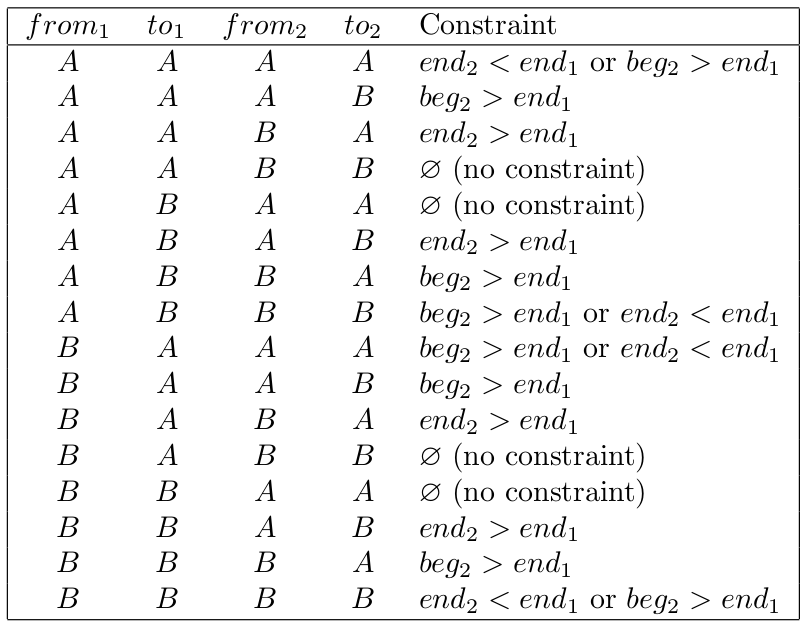
\includegraphics[width=8cm]{rest}
        \caption{Restricciones de orden en pistas simples (Fuente \cite{Problem})}
        \label{fig:rest}
        \end{figure}


        \item \textbf{Conflictos en grupos de pistas.}
        \begin{align*}
            \mathcal{M} &:= \text{Conjunto de movimientos posibles en grupos de pistas}.\\
            \text{hwTime}_k &:= \ \text{Tiempo de seguridad mínimo entre trenes en } k \in \mathcal{K}. \\
            \text{ind}_g &:= \ \text{Indice de puerta para un lado de } k \in \mathcal{K}.
        \end{align*}
        Existen dos posibles casos de conflictos. Primero, cuando dos trenes van en la misma dirección:
        \begin{align*}
            \forall (m_1,m_2,k) \in \mathcal{M}\times \mathcal{K}, \text{ con } \text{side}_{o_1} = \text{side}_{o_2}, \\
            (\text{ind}_{o_1}-\text{ind}_{o_2})\times (\text{ind}_{d_1}-\text{ind}_{d_2}) \leq 0 \Rightarrow |h_1-h_2| \geq \text{hwTime}_k,
        \end{align*}
        y cuando los trenes van en direcciones opuestas:
        \begin{align*}
            \forall (m_1,m_2,k) \in \mathcal{M}\times \mathcal{K}, \text{ con } \text{side}_{o_1} \neq \text{side}_{o_2}, \\
            (\text{ind}_{o_1}-\text{ind}_{d_2})\times (\text{ind}_{d_1}-\text{ind}_{o_2}) \leq 0 \Rightarrow |h_1-h_2| \geq \text{trTime}_k \text{hwTime}_k.
        \end{align*}



        \item \textbf{Capacidad de estacionamientos.} La capacidad de las vías de estacionamiento debe ser respetada:
        \begin{align*}
            \forall y \in \mathcal{Y}, \forall h \in \mathcal{H}, \text{nbTrain}_{y,h} \leq \text{capa}_y.
        \end{align*}
    \end{enumerate}

\end{description}

\subsection{Función Objetivo}
    La función objetivo corresponde a múltiples objetivos, asociados a penalizaciones por violación de situaciones insatisfactorias, cuyo objetivo es minimizar. Esta se modela como una suma con pesos del siguiente modo:
    \begin{align}
     f = w_1 f^{\text{uncov}} + w_2 f^{\text{maint}} + w_3 f^{\text{plat}} + w_4 f^{\text{pref}} + w_5 f^{\text{reuse}}
     \label{eq:objetivo}    
    \end{align}
    donde cada término de (\ref{eq:objetivo}) se detalla a continuación. Los pesos $w_i$ de la suma se definen en razón de la importancia que se le quiere dar a cada término. Por lo general peso dominante es $w_1$, pues se quiere evitar en gran medida que llegadas/salidas queden sin cubrir.

    \begin{enumerate}
        \item \textbf{Llegadas/Salidas sin cubrir.} También incluye el costo por no usar trenes inicialmente en el sistema. Si para cada una de estas situaciones (LLegadas o salidas sin cubrir, o trenes iniciales no utilizados) se define un costo unitario $\text{uncovCost}$, entonces el costo puede expresarse como:
        \begin{align*}
            f^{\text{uncov}} = \text{uncovCost} \times \left( \left| \{t \in \mathcal{T} \setminus \mathcal{T}^+\} \right| + \left| \{ d \in \mathcal{D}: \text{depTrain}_d = \emptyset \} \right| \right)
        \end{align*}
        \item \textbf{Costos por sobre mantención.} Este costo va asociado a la realización de mantenciones (Tipo D y T), sobre trenes que aún tiene capacidad para seguir viajando $\text{remTBM} > 0$ y $\text{remDBM} > 0$. Para ellos se definen los costos unitarios $\text{remDCost}$ y $\text{remTCost}$, por cada unidad de TBM y DBM que no se utiliza al realizar la mantención respectiva. Luego el costo total queda:
        \begin{align*}
            f^{\text{maint}} = \sum_{\substack{e \in \mathcal{E} \\ c_e = \text{D} \\y_e = \text{\texttt{BegMaintenance}}}} \text{remDCost}\times \text{remDBM}_{t_e} + \sum_{\substack{e \in \mathcal{E} \\ c_e = \text{T} \\y_e = \text{\texttt{BegMaintenance}}}} \text{remTCost}\times \text{remTBM}_{t_e}.
        \end{align*}

        \item \textbf{Costo por uso de plataformas.} Como se mencionó anteriormente, aquí hay tres posibilidades. Que una llegada ocupe la plataforma (llamamos a este conjunto $\mathcal{A}' \subset \mathcal{A}$), que una salida ocupe la plataforma $\mathcal{D}' \subset \mathcal{D}$ o que una llegada seguida inmediatamente por una salida ocupe esta plataforma (llamaremos a este conjunto $\mathcal{Z} \subset \mathcal{A}\times \mathcal{D}$). Adicionalmente se define las variables $\text{dwell}_a$, $\text{dwell}_d$ y $\text{dwell}_z$, el tiempo de la plataforma que se asigna a cada una de estas posibilidades. Naturalmente se define $\text{idealDwell}_z = \text{idealDwell}_a + \text{idealDwell}_d$ con $z=(a,d)$. Luego, una penalización $\text{dwellCost}$ es aplicada por cada unidad de tiempo que se realice sobre el tiempo ideal, en cada caso. Esto se expresa para cada caso como sigue:
        \begin{align*}
            f^{\text{plat}_1} &= \sum_{a \in \mathcal{A}^*} \text{dwellCost}\times |\text{dwell}_a - \text{idealDwell}_a| \\
            f^{\text{plat}_2} &= \sum_{d \in \mathcal{D}^*} \text{dwellCost}\times |\text{dwell}_d - \text{idealDwell}_d| \\
            f^{\text{plat}_3} &= \sum_{z \in \mathcal{Z}} \text{dwellCost}\times |\text{dwell}_z - \text{idealDwell}_z|,
        \end{align*}
        siendo la función de costo general: $f^{\text{plat}} = f^{\text{plat}_1} + f^{\text{plat}_2} + f^{\text{plat}_3}$.

        \item \textbf{Costo por no satisfacer preferencia de plataformas.} Si tanto para las llegadas $a \in \mathcal{A}$, como las salidas $d \in \mathcal{D}$ se aplica un costo por no asignar una de las plataformas preferidas: $\text{platAsgCost}$. Entonces el costo general queda:
        \begin{align*}
            f^{\text{pref}} = \sum_{\substack{a \in \mathcal{A} \\  \text{plat}_a \notin \text{prefPlat}_a}} \text{platAsgCost} + \sum_{\substack{d \in \mathcal{D} \\  \text{plat}_d \notin \text{prefPlat}_d}} \text{platAsgCost}
        \end{align*}


        \item \textbf{Costo por no satisfacer reusos.} Sea $\text{reuseCost}$ el costo asociado a no satisfacer cualquier reuso $u \in \mathcal{U}$, luego el costo general es:
        \begin{align*}
             f^{\text{reuse}} = \sum_{\substack{u \in \mathcal{U} \\ \text{depTrain}_{\text{dep}_u}\neq \text{arrTrain}_{\text{arr}_u}}} \text{reuseCost}.    
        \end{align*}
    \end{enumerate}


\section{Representación}

Tal como lo propuso Haarh et al. \cite{MathHeuristic}, el problema se abordó subdividiendo en tres subproblemas más simples de resolver. El primero de ellos corresponde al \textit{Matching} entre las salidas y los trenes en el sistema (trenes asociados a llegadas o inicialmente en el sistema). Una vez conocidos que trenes cubriran qué salidas, es posible abordar el problema de \textit{Platform Assignment}, el que consiste en asignar una plataforma a todas las llegadas y salidas por cubrir, esto es, si en la fase anterior se determinó no cubrir una salida entonces no debe ser considerada para una plataforma. Con las secuencias de entrada y salida \textit{fijas} y las asignaciones anteriores cubiertas, queda por resolver el problema de \textit{Routing} de cada tren dentro de la estación, es decir, la ruta de recursos por los que pasa y utiliza entre su llegada y su próxima salida, más las secuencias de puertas de los \textit{Track Groups} que utiliza en sus secuencias de entrada y salida. A continuación se detalla la representación utilizada para cada caso, más la representación utilizada para manejar todos los datos de cada instancia.

\begin{description}
    \item[\textsc{Instancias.}] Para manejar cada tabla correspondiente a una instancia, se decidió utilizar diccionarios del siguiente tipo:
    \begin{flalign*}
        \texttt{TableName[keyId]} = \texttt{valueStruct}
    \end{flalign*}
    donde \texttt{keyId} es el ID primario de la tabla, y \texttt{valueStruct} es una estructura para contener el resto de campos de cada fila. Para la implementación de cada diccionario se utiliza \textit{ordered map} \cite{OrdMap}, que internamente mantiene los datos en una estructura de árbol que preserva el orden de los elementos, lo cual es útil pues se requiere iterar en orden sobre estas estructuras. Se elige esta representación por el fácil manejo de datos que permite, muy similar al acceso en tablas.

    \item[\textsc{Matching.}] Un matching consiste básicamente en un par \textit{Departure}-\textit{Train}, con el tren asociado a cada uno de los \textit{departures}. Por lo mismo, se propone utilizar también una estructura de diccionario del siguiente tipo:
    \begin{flalign*}
         \texttt{Matches[departureId]} = \texttt{trainId}
     \end{flalign*}
     donde \texttt{departureId} y \texttt{trainId} son los IDs de la salida y del tren respectivamente. Debido a que sobre estas estructuras se requiere realizar gran cantidad de consultas y modificaciones (operaciones \textit{insert}), se utiliza un \texttt{unordered map} \cite{UnOrdMap}, que internamente accede a los datos por una \textit{tabla hash} cargada en memoria, lo cual produce tiempos de inserción y búsqueda constantes, siendo por tanto una solución eficiente.

    \item[\textsc{Platform Assignment.}] Una asignación de plataforma consiste en un par \textit{Arrival}-\textit{Platform} o \textit{Departure}-\textit{Platform}. Por lo tanto, al igual que en el caso anterior se utiliza un diccionario del siguiente tipo:
    \begin{align*}
        \texttt{Assignment[arrivalId || departureId]} = \texttt{platformId}
    \end{align*}
    donde la llave del diccionario pueden ser \texttt{arrivalId} (ID de llegada) o \texttt{departureId} (ID de salida), y \texttt{platformId} el ID de la plataforma asignada. Para la implementació se ocupa un \textit{unsorted map} al igual que en el anterior.

    \item[\textsc{Routing.}] Cada pasada que realiza un tren por un recurso de la estación se caracteriza por lo siguiente:
    \begin{align*}
        \texttt{passStruct} = [\texttt{indexGate}_a, \texttt{ResourceId}, \texttt{indexGate}_b, \texttt{direction}, \texttt{entryTime}, \texttt{exitTime}]
    \end{align*}
    donde $\texttt{indexGate}_a$ e $\texttt{indexGate}_b$ son los indices de las puertas de los lados A y B respectivamente, \texttt{ResourceId} es el ID del recurso utilizado,  \texttt{direction} es un \texttt{flag} para indicar en qué dirección se cruza el recurso: $\texttt{A}\rightarrow \texttt{B}$ ó $\texttt{A}\leftarrow \texttt{B}$ y \texttt{entryTime} y \texttt{exitTime} son los tiempos de entrada y salida del recurso respectivamente.

    Luego para representar la ruta de cada tren se usa una \textbf{lista dinámica} de tales estructuras, pues el largo y tipo de recursos de cada ruta puede ir cambiando en la solución. Notar que esta representación es fácilmente transformable a la representación de solución propuesta en el problema original \cite{Problem}.
\end{description}

\section{Descripción del Algoritmo}

Siguiendo las mismas ideas anteriores, se procede a explicar el algoritmo utilizado para resolver cada uno de los subproblemas. Para la resolución de tales subproblemas (dada su conocida y estudiada complejidad), se propone ocupar el método \textit{heurístico} Tabu Search, con las adaptaciones para los movimientos que generan la vecindad correspondientes.

\begin{description}
    \item[\textsc{Matching.}] La idea es mantener (en la medida de lo posible) las soluciones dentro de la zona de factibilidad, por ello dos \textit{departures} distintos no pueden tener asociado el mismo tren en el diccionario $\texttt{Matches[departureId]}=\texttt{trainId}$. Otra situación infactible se da cuando el tren asociado llega a la estación después de tal salida, sin embargo cuando existan tales asignaciones se considerará esa salida como no cubierta, y se penalizará con un costo \texttt{uncovCost}.

    Para generar la vecindad, se itera sobre cada uno de los \texttt{departureId} en \texttt{Matches} siguiendo el siguiente procedimiento:
    \begin{enumerate}
        \item Se genera un \texttt{trainId} aleatorio entre los IDs de todos los trenes de la estación (trenes iniciales y de llegadas).
        \item Si tal \texttt{trainId} ya está asignado a otro \textit{departure} se aplica un \textit{swap} entre las asignaciones.
        \item De otro modo se aplica un \textit{insert}, asignando el \texttt{trainId} generado al \textit{departure}.
    \end{enumerate}
    Tales movimientos permiten mantener soluciones factibles, y al mismo tiempo ir incorporando distintas combinaciones. Entre los vecinos generados, se evalúan los costos por medio de las asignaciones insatisfechas descritas recién (\texttt{uncovCost}) y los reusos no satisfechos (\texttt{reuseCost}). El vecino con menor costo es seleccionado como la solución actual, y se agregan las asignaciones anteriores a un diccionario $\texttt{Tabu[departureIdPrev]}=\texttt{trainIdPrev}$. En Algorithm \ref{first} se resume el movimiento generador de la vecindad.

\begin{algorithm}
\caption{Generador de vecindad para \textit{Matching problem}}\label{first}
\begin{algorithmic}[1]
\Procedure{neighborhood}{\texttt{Matches}}
\State{\texttt{Matches} = \texttt{Matches.copy()}}
\State{\texttt{bestNeigh} = \texttt{Matches.copy()}}
\For{\texttt{depId},\texttt{trId} in \texttt{Matches.items()}}
\State{\texttt{ntrId} = \texttt{generateRandomTrainId()}}
\If{\texttt{ntrId} \texttt{in} \texttt{Matches.values()}}
\State{\texttt{ndepId} = \texttt{Matches.findkey(ntr)}}
\State{\texttt{Matches[depId]} = \texttt{ntrId}}
\State{\texttt{Matches[ndepId]} = \texttt{trId}}
\Else
\State{\texttt{Matches[depId]} = \texttt{ntrId}}
\EndIf
\If{\texttt{cost(Matches)} $<$ \texttt{cost(bestNeigh)}}
\State{\texttt{bestNeigh} = \texttt{Matches}}
\EndIf
\State{\texttt{undoModification(Matches)}}
\EndFor
\EndProcedure
\end{algorithmic}
\end{algorithm}


    \item[\textsc{Platform Assignment.}] Para las asignaciones de plataforma hay $3$ principales restricciones: (1) Preferencias de plataforma (blanda), (2) Capacidad de plataformas (dura), (3) Recursos usados con anterioridad (dura). Adicionalmente cada llegada y salida no puede tener asignada más de una plataforma, pero dada la representación de la solución esto no se puede dar. La restricción (1) se agrega como costo de penalización (\texttt{platAsgCost}), del mismo modo que (2) a pesar de ser restricción dura, pues no es trivial producir movimientos que la mantengan satisfecha. Sin embargo por cada plataforma que viole su capacidad, se aplica un costo de $N \cdot \texttt{platAsgCost}$, con $N$ definido por el usuario. Si un movimiento genera una solución que viole (3), entonces se descarta.

    El movimiento en cuestión es una simplificación del anterior. Sobre cada uno de los \texttt{arrivalId} o \texttt{departureId} en \texttt{Assignment}:
    \begin{enumerate}
           \item Se genera un \texttt{plataformId} aleatorio entre los IDs de todas las plataformas.
           \item Se aplica un \textit{insert}, asociando tal plataforma al \textit{arrival} o \textit{departure} en cuestión.
    \end{enumerate}
    En algorithm \ref{second} se resume el movimiento generador de la vecindad.

    \textbf{Observación:} Para determinar que dos eventos (\textit{arrival} o \textit{departure}) estan haciendo uso de la misma plataforma al mismo tiempo, se verifica si hay intersección de los intervalos $[\texttt{arrivalTime},\texttt{arrivalTime}+\texttt{maxDwellTime}]$ o $[\texttt{departureTime},\texttt{departureTime}+\texttt{maxDwellTime}]$ respectivamente. Considerar tales asignaciones con el máximo tiempo que se puede estar en plataforma da más holgura a la fase de routing.
\begin{algorithm}
\caption{Generador de vecindad para \textit{Platform Assignment Problem}}\label{second}
\begin{algorithmic}[1]
\Procedure{neighborhood}{\texttt{Assignment}}
\State{\texttt{Assignment} = \texttt{Assignment.copy()}}
\State{\texttt{bestNeigh} = \texttt{Assignment.copy()}}
\For{\texttt{eventId},\texttt{platId} in \texttt{Assignment.items()}}
\State{\texttt{nplatId} = \texttt{generateRandomPlatformId()}}
\State{\texttt{Assignment[eventId]} = \texttt{nplatId}}
\If{\texttt{cost(Assignment)} $<$ \texttt{cost(bestNeigh)}}
\State{\texttt{bestNeigh} = \texttt{Assignment}}
\EndIf
\State{\texttt{undoModification(Assignment)}}
\EndFor
\EndProcedure
\end{algorithmic}
\end{algorithm}


    

    \item[\textsc{Routing.}] Una vez conocidas las asignaciones anteriores, basta por conocer el itinerario o ruta que sigue cada tren dentro de la estación. Como se dijo anteriormente, la ruta está compuesta por la secuencia de entrada (fija), la \textit{secuencia intermedia} (no determinada) y la secuencia de salida (fija). Se le llama secuencia intermedia  a la ruta que sigue el tren entre su llegada y su próxima salida. De las secuencias de llegada/salida lo único que se puede decidir, son la combinaciones de \textit{gates} utilizadas para atravesar los trackgroups, y los tiempos respectivos. En cambio para las secuencias intermedia existe mayor flexibilidad.

    El movimiento propuesto para generar una vecindad de soluciones, consiste en seleccionar aleatoriamente (para un tren particular) que secuencia modificar (entrada, intermedia o salida). Luego se sigue del siguiente modo:
    \begin{enumerate}
        \item (\textit{Secuencia de entrada}.) Para cada \textit{Track Group} en la secuencia de entrada, genera aleatoriamente una combinación de puertas $(\texttt{indexGate}_a, \texttt{indexGate}_b)$.

        \item (\textit{Secuencia Intermedia}.) Dada un secuencia intermedia de eventos $\texttt{seqInter}$ de largo $M$, en primer lugar se determinan una subsección (aleatoria) de tal secuencia $\texttt{seqInter}[i:j]$, entre los eventos $1 \leq i$ y $j \leq M$. Sean $\texttt{Resource}[i]$ y $\texttt{Resource}[j]$ los recursos al extremo de tal subsección, se elige (aleatoriamente) una subsección distinta con los mismo recursos extremos, que calce con los tiempos \texttt{entryTime} y \texttt{exitTime} respectivos.  

        \item (\textit{Secuencia de Salida}.) Del mismo modo que en la entrada, para cada \textit{Track Group} en la secuencia de salida, genera aleatoriamente una combinación de puertas $(\texttt{indexGate}_a$, $\texttt{indexGate}_b)$.
    \end{enumerate}
    \textbf{Observaciones:} (1) Para los movimientos de secuencias de entrada/salida no se modifican los tiempos, dado que el tiempo para atravesar cada \textit{track group} es fijo e igual a \texttt{trTime}. (2) Los movimientos de secuencias intermedias suponen que se tienen \textit{precomputadas} todas las posibles rutas entre dos recursos de la estación, lo que en la práctica puede ser un número muy elevado. En tal caso, siempre es posible trabajar con un subconjunto \textit{más razonable} de tales rutas.
\end{description}

\section{Experimentos}

En lo que sigue se refiere sólo a los primeros dos subproblemas, dado que la implementación del algoritmo propuesto para resolver el problema de \textit{Routing} mostró no ser efectivo, debido a la gran cantidad de combinaciones de subsecciones intermedias posibles entre dos recursos dados, y que la mayoría de estos se encuentran en la zona de no factibilidad.

Para generar las pruebas $10$ instancias fueron ocupadas \footnotemark[1], ordenadas por orden de dificultad y correspondientes a versiones simplificadas de las utilizadas en el concurso \textit{ROADEF/EURO Challenge 2014}. En particular, sólo se considera un día de horizonte de planificación, todos los recursos y salidas son compatibles con todos los trenes, el $\texttt{remDBM} > \texttt{reqDBM}$ (lo mismo para el tiempo) y no existen llegadas ni salidas conjuntas.

A continuación se detallan configuraciones propias para cada subproblema tratado.

\begin{description}
    \item[\textsc{Matching.}] Se tienen aquí dos principales parámetros: \texttt{numIterTabu} (número de iteraciones de Tabu Search) y \texttt{tabuLength} (largo máximo de la lista Tabú). Para obtener los mejores resultados se realiza un sintonización \textit{manual} de parámetros. Debido a la naturaleza aleatoria de los movimientos que genera la vecindad, una misma configuración de parámetros no siempre entrega el mismo resultado, por lo que en algunos casos fue necesario repetir las pruebas varias veces con la misma configuración.
    \item[\textsc{Platform Assignment.}] Los parámetros principales son los mismos: \texttt{numIterTabu} (número de iteraciones de Tabu Search) y \texttt{tabuLength} (largo máximo de la lista Tabú), más el peso asociado para castigar las violaciones de capacidad en las plataformas, determinadas por $N: \ N \cdot \texttt{platAsgCost}$. Igual que para el caso anterior, una sintonización manual fue realizada con repeticiones para contrarrestar los efectos de la aleatoriedad. Después de pruebas en varias instancias, se determinó que un valor razonable para $N$ es entre $[5,10]$ (el valor ocupado en los experimentos siguientes es $5$).  
\end{description}

\footnotetext[1]{\url{http://csrg.cl/~mavillan/instances/}}

\section{Resultados}

\begin{description}
    \item[\textsc{Matching.}] Como se indicó anteriormente, un proceso de sintonización de parámetros fue realizado para tener buenos resultados en cada instancia. En general el parámetro más determinante en este caso es el número de iteraciones a realizar, de modo que a medida que aumenta la complejidad de las instancias, más iteraciones son requeridas. Para el largo de la lista Tabú fue utilizado el siguiente criterio: $\texttt{tabuLength}=\texttt{numIterTabu}/10$ obteniendo buenos resultados. En Cuadro 1 se muestran los resultados para la instancia $4$ con $\texttt{numIterTabu}=1000$ y $\texttt{tabuLength}=10$, obteniendo una solución óptima.
\begin{table}[htpb!]
\centering
\label{tab:1}
\begin{tabular}{|l|l|}
\hline
\rowcolor[HTML]{329A9D}
\textbf{DepartureID}         & \textbf{TrainID}               \\ \hline
{\color[HTML]{000000} Dep1}  & {\color[HTML]{000000} Train12} \\ \hline
{\color[HTML]{000000} Dep2}  & {\color[HTML]{000000} Train2}  \\ \hline
{\color[HTML]{000000} Dep3}  & {\color[HTML]{000000} Train13} \\ \hline
{\color[HTML]{000000} Dep4}  & {\color[HTML]{000000} Train4}  \\ \hline
{\color[HTML]{000000} Dep5}  & {\color[HTML]{000000} Train5}  \\ \hline
{\color[HTML]{000000} Dep6}  & {\color[HTML]{000000} Train6}  \\ \hline
{\color[HTML]{000000} Dep7}  & {\color[HTML]{000000} Train7}  \\ \hline
{\color[HTML]{000000} Dep8}  & {\color[HTML]{000000} Train8}  \\ \hline
{\color[HTML]{000000} Dep9}  & {\color[HTML]{000000} Train9}  \\ \hline
{\color[HTML]{000000} Dep10} & {\color[HTML]{000000} Train10} \\ \hline
\end{tabular}
\caption{Ejemplo de Matching (instancia 4) - \texttt{MinObjFunc} = 0}
\end{table}

    Todas las instancias pudieron ser resueltas con $\texttt{MinObjFunc}=0$. Para las instancias pequeñas con $100$ iteraciones fue suficiente, mientras que para las más grandes fueron necesarias $\sim5000$ para alcanzar una \textit{match} óptimo. En Figura \ref{fig:minobj2} se muestran los resultados sobre la instancia $10$ para distintos números de iteraciones, y ocupando $\texttt{tabuLength}=\texttt{numIterTabu}/10$. 

    \begin{figure}[htpb!]
    \centering
    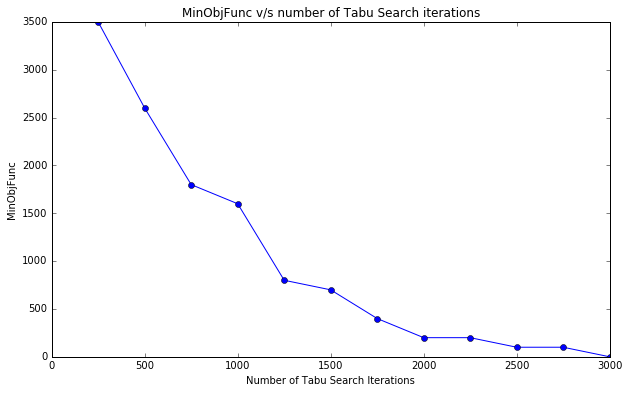
\includegraphics[width=11cm]{minobjfunc2}
    \caption{\texttt{MinObjFunc} para instancia $10$ a distinto número de iteraciones (Fuente \cite{Higgins})}
    \label{fig:minobj2}
    \end{figure}

    \item[\textsc{Platform Assignment.}] Al igual que el caso anterior, en primer lugar se realizó un proceso de sintonización de parámetros. Sin embargo este problema resultó más complejo de resolver que el anterior, no obteniendo soluciones perfectas para cada instancia. En \ref{table2} se muestran los resultados sobre la instancia $4$ con $\texttt{numIterTabu}=1000$ y $\texttt{tabuLength}=100$, para lo cual no se obtiene una asignación perfecta, debido a dos \textit{reusos} no satisfechos.
\begin{table}[htpb!]
\centering
\label{table2}
\begin{tabular}{|c|c|}
\hline
\rowcolor[HTML]{329A9D}
\textbf{{[}Arrival/Departure{]}ID} & \textbf{PlaformID} \\ \hline
Arr10                              & Platform4          \\ \hline
Arr12                              & Platform2          \\ \hline
Arr13                              & Platform8          \\ \hline
Arr2                               & Platform6          \\ \hline
Arr4                               & Platform5          \\ \hline
Arr5                               & Platform3          \\ \hline
Arr6                               & Platform5          \\ \hline
Arr7                               & Platform7          \\ \hline
Arr8                               & Platform8          \\ \hline
Arr9                               & Platform2          \\ \hline
Dep1                               & Platform6          \\ \hline
Dep10                              & Platform5          \\ \hline
Dep2                               & Platform5          \\ \hline
Dep3                               & Platform7          \\ \hline
Dep4                               & Platform9          \\ \hline
Dep5                               & Platform9          \\ \hline
Dep6                               & Platform6          \\ \hline
Dep7                               & Platform6          \\ \hline
Dep8                               & Platform8          \\ \hline
Dep9                               & Platform5          \\ \hline
\end{tabular}
\caption{Ejemplo de Platform Assignment - \texttt{MinObjFunc} = 200}
\end{table}    
El comportamiento que sigue este problema es similar al anterior; Para obtener buenos resultados en las instancias más complicadas es necesario iterar una mayor cantidad de veces.

    En la figura \ref{fig:minobj} se muestran los valores mínimos de la función objetivo \texttt{MinObjFunc} para cada una de las $10$ instancias, con \texttt{numIterTabu}$=10000$ y \texttt{tabuLength}$=100$.
    \begin{figure}[htpb!]
    \centering
    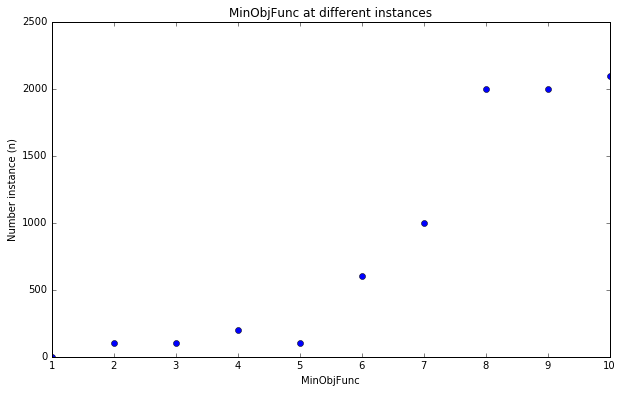
\includegraphics[width=11cm]{minobjfunc}
    \caption{\texttt{MinObjFunc} para \texttt{numIterTabu}=10000 y \texttt{tabuLength}=100 (Fuente \cite{Higgins})}
    \label{fig:minobj}
    \end{figure}
    claramente el problema es mucho más complicado de resolver en instancias mayores, habiendo una gran cantidad preferencias de plataforma insatisfechas.
\end{description}




\newpage
\section{Conclusiones} \label{conclusions}

\large{\textbf{{\textsc{Conclusiones acerca del Estado del Arte}}}}\\

El estudio realizado en el presente documento, ha analizado a cabalidad el problema propuesto en ROADEF/EURO Challenge 2014 desde distintos enfoques. En base a esto se puede observar que la innovación que propone este problema, es modelar todas las operaciones que se realizan en una estación de una manera holística, y no cómo varios subproblemas más pequeños, que es lo que se ha venido haciendo desde antes. Sin embargo tal formulación, trae como consecuencia un problema extremadamente complejo. Esto se verifica en que para instancias reales, es totalmente infactible obtener una solución exacta, y es más, al día de hoy existen instancias para las cuales no se sabe (no se ha encontrado) ninguna asignación que deje sin cubrir alguna llegada o salida.

La verdadera dificultad del problema se puede verificar, viendo que tan sólo una versión simplificada de uno de sus subproblemas, el \textit{Timetable Scheduling Problem} (TSP) en un sóla vía, ha demostrado ser NP-\textit{hard} (en el sentido estricto) \cite{Caprara}.

En virtud de tal dificultad, la mayoría de los trabajos relacionados que se estudiaron, tratan de desacoplar de alguna forma el problema original, para resolver subproblemas más simples. En general el enfoque más seguido es tratar el problema original en dos partes: En primer lugar determinan las posibles \textbf{asignaciones} de trenes para las salidas, y en segundo lugar se intentan computar las \textbf{rutas} que deben seguir los trenes entre los recursos de la estación, sin violar las restricciones. Es decir, el desacople consiste en tratar un problema de asignación y otro de enrutamiento.

Debido al inviabilidad de utilizar métodos exactos para computar la solución, la mayoría de enfoques que han tenido éxito han sido aquellos que han utilizado heurísticas, para así al menos generar soluciones aproximadas. En particular, tal como reporta \cite{Higgins}, la combinación de distintas heurísticas ha probado ser muy efectiva.  Debido a la gran cantidad de variables que posee el problema, y al tamaño del espacio de búsqueda, otro método que ha resultado útil ha sido el de generación de columnas. Es importante indicar, que pese a que los métodos exactos no son útiles para el problema general, estos sí han sido utilizados en subproblemas específicos. Tal es el caso de \textit{Branch and Bound} en \cite{DAriano}.

Para finalizar este estudio del \textit{estado del arte}, se hace un énfasis en que la mayoría de los autores estudiados, indican que sus métodos y algoritmos tienen muchas variantes por probar y mejorar, por lo tanto las posibilidades de resolver instancias cada vez más grandes, y obtener buenas soluciones están abiertas. \\


\large{\textbf{{\textsc{Conclusiones acerca de la Implementación}}}}\\

La Heurística \textit{Tabu} search mostró un comportamiento bastante bueno en la resolución de los dos primeros subproblemas tratados: \textit{Matching Problem} y \textit{Platform Assignment Problem}. Para el primero los resultados son notablemente buenos, pudiendo resolver todas las instancias de forma óptima en una cantidad razonable de iteraciones del algoritmo. Como se hizo notar, con $\sim 5000$ iteraciones fue posible resolver hasta las instancias más complejas del problema de forma óptima. Sin embargo para número inferiores de iteraciones, pese a no tener una solución óptima se generan soluciones subóptimas bastante aceptables. Esto es un gran aporte para casos de instancias reales, en donde aplicar técnicas completas resulta totalmente inviable, y por lo tanto la única alternativa es ocupar técnicas basadas en Heurísticas para acercarse de algún modo al óptimo.

Otro aspecto importante a notar, es que dado que la lista Tabú (que en verdad es un diccionario) posee una estructura simple, y sólo almacena los pares de asignaciones utilizadas anteriormente, es que entonces es posible manejar listas de gran tamaño sin requerir de un costo computacional elevado, ni de gran uso de memoria.

Para el segundo subproblema no se obtienen tan buenos resultados como en el caso anterior, pero de todos modos son aceptables. Los costos reportados en la función objetivo, son mayormente debido las preferencias de plataformas insatisfechas. Esto se debe  a que, cómo se formuló el problema, la penalización por exceder la capacidad de una plataforma es mucho mayor que no satisfacer preferencias. Por otro lado, los recursos consumidos con anterioridad no aportan a la función objetivo, pues la soluciones que violan tales restricciones son simplemente descartadas. Probablemente un movimiento más elaborado que el \textit{insert} propuesto permitiese generar mejores vecindarios, y sería una propuesta interesante de estudiar. Adicionalmente, para verificar el exceso de capacidad de una plataforma se toma una ventana de tiempo \textit{pesimista}, en el sentido que se supone que cada tren estará el máximo de tiempo posible en la plataforma. Este criterio puede ser muy duro, y probablemente es una de las causales de que no se puedan llegar a mejores soluciones.

El tercer subproblema \textit{Routing problem}, resultó ser el más complicado de formular y resolver. La mayor complicación se encontró en la determinación de soluciones vecinas (que fuesen cercanas de algún modo) para la aplicación de Tabu Search. El algoritmo propuesto para la generación de secuencias intermedias es interesante, pero muy poco práctico, pues requiere de manejar una gran cantidad de combinaciones entre rutas que unen dos recursos dados, siendo algunas de estas rutas \textit{poco coherentes}. Una posible mejora a tal proceso, es un generación manual de rutas \textit{coherentes} y \textit{viables} entre dos recursos dados, ahorrandole así al algoritmo probar soluciones que no tienen mucho sentido, o que son del todo infactibles. Tal idea no es tan \textit{descabellada} si se tiene en cuenta que se debe realizar una sola vez, puesto que raramente la estructura de los recursos de una estación de trenes se ve modificada.





\newpage
\section{Bibliografía}

\bibliographystyle{unsrt}
\bibliography{referencias}

\end{document}


